\documentclass[11pt, a4paper]{article}

% Legger inn pakker som skal brukes:	
\usepackage[utf8]{inputenc}
\usepackage{color}

\usepackage{titlesec}

\usepackage{amsmath}
\usepackage{float}
\usepackage[export]{adjustbox}
\usepackage[hidelinks]{hyperref}
\numberwithin{figure}{section}
\numberwithin{table}{section}	
\usepackage{graphicx}
\usepackage{subcaption}
\usepackage{verbatim}
\usepackage{float}
\graphicspath{{bilder/}}
\usepackage{verbatim}
\usepackage{etoolbox}
\usepackage{tabularx}
\usepackage[margin=2.54cm]{geometry}
\usepackage[british]{babel}
\usepackage[backend=biber, style=ieee, dashed=false]{biblatex}
\bibliography{referencelist.bib}
\usepackage{setspace}
\usepackage{csquotes}
\usepackage[titletoc]{appendix}
\usepackage{listings}
\usepackage{enumitem}
\usepackage{environ}

\definecolor{dkgreen}{rgb}{0,0.6,0}
\definecolor{gray}{rgb}{0.5,0.5,0.5}
\definecolor{mauve}{rgb}{0.58,0,0.82}

\lstset{frame=tb,
  language=Python,
  aboveskip=3mm,
  belowskip=3mm,
  showstringspaces=false,
  columns=flexible,
  basicstyle={\small\ttfamily},
  numbers=none,
  numberstyle=\tiny\color{gray},
  keywordstyle=\color{blue},
  commentstyle=\color{dkgreen},
  stringstyle=\color{mauve},
  breaklines=true,
  breakatwhitespace=true,
  tabsize=3
}

% Makro definisjoner
\newcommand{\code}[1]{\texttt{#1}}

%Usermanual setup found on this page: https://tex.stackexchange.com/a/130099 URL visited 10.05.2019
%code starts here
\newlength\widest
\makeatletter

\NewEnviron{userManualItemlist}{%
  \vbox{%
    \global\setlength\widest{0pt}%
    \def\item[##1]{%
      \settowidth\@tempdima{\textbf{##1}}%
      \ifdim\@tempdima>\widest\global\setlength\widest{\@tempdima}\fi%
    }%
    \setbox0=\hbox{\BODY}%
  }
  \begin{description}[
    leftmargin=\dimexpr\widest+0.5em\relax,
    labelindent=0pt,
    labelwidth=\widest]
  \BODY
  \end{description}%
}
\makeatother
%code ends here

\begin{document}

	% Front page
	\begin{titlepage}
	\noindent\begin{tabularx}{\textwidth}{ |X|>{\centering}X| }
  		\hline
		\multicolumn{2}{|X|}{} \tabularnewline
  		\multicolumn{2}{|>{\centering\hsize=\dimexpr2\hsize+2\tabcolsep+\arrayrulewidth\relax}X|}{
\includegraphics[scale=0.1]{uis_logo}} \tabularnewline
		\multicolumn{2}{|X|}{} \tabularnewline
		\multicolumn{2}{|>{\centering\hsize=\dimexpr2\hsize+2\tabcolsep+\arrayrulewidth\relax}X|}{{\fontsize{10}{12}\selectfont\textbf{Faculty of Science and Technology}}} \tabularnewline 
		\multicolumn{2}{|X|}{} \tabularnewline
		\multicolumn{2}{|>{\centering\hsize=\dimexpr2\hsize+2\tabcolsep+\arrayrulewidth\relax}X|}{{\fontsize{16}{19.2}\selectfont\textbf{BACHELOR'S THESIS}}} \tabularnewline
		\multicolumn{2}{|X|}{} \tabularnewline
  		\hline
		Study program/Specialization: & \tabularnewline
		 & Spring 6th semester, 2019 \tabularnewline
		 & \tabularnewline
		Computer Science & Open \tabularnewline % TODO finne ut om den skal være åpen eller konfidensiell
		 & \tabularnewline
		\hline
		Writer(s): & Signature \tabularnewline
		 & \tabularnewline
		Christoffer Holmesland & ................................................ \tabularnewline % TODO legg til signaturer
		 & \tabularnewline
		Jørgen Melstveit & ................................................ \tabularnewline
		 & \tabularnewline
		Gaute Haugen & ................................................ \tabularnewline
		 & \tabularnewline
		 & \tabularnewline
		\hline
		\multicolumn{2}{|X|}{Facalty supervisor: Erlend Tøssebro} \tabularnewline
		\multicolumn{2}{|X|}{} \tabularnewline
		\multicolumn{2}{|X|}{} \tabularnewline
		\multicolumn{2}{|X|}{} \tabularnewline
		\hline
		\multicolumn{2}{|>{\setlength\hsize{2\hsize}}X|}{Thesis title: Web application + mobile application for use in interactive teaching - DAT200 and DAT110} \tabularnewline
		\multicolumn{2}{|X|}{} \tabularnewline
		\multicolumn{2}{|X|}{} \tabularnewline
		\hline
		\multicolumn{2}{|>{\setlength\hsize{2\hsize}}X|}{Number of credits: 20} \tabularnewline
		\multicolumn{2}{|X|}{} \tabularnewline
		\hline
		Key words: &  \tabularnewline
		 & Pages:  \tabularnewline % TODO legg til antall sider
		 & \tabularnewline
		 & + enclosure:  \tabularnewline % TODO legg til vedlegg/annet
		 & \tabularnewline
		 & Stavanger, 15/05-2018 \tabularnewline
		 & \tabularnewline
		\hline
	\end{tabularx}
	\vspace{0.3cm}
	\begin{center}
		{\fontsize{10}{12}\selectfont Frontpage for bachelor thesis \\
		Faculty of Science and Technology}
	\end{center}	
\end{titlepage}

	\begin{spacing}{1.25}
		% Table of contents
		\renewcommand{\contentsname}{Table of Contents}
\tableofcontents
\thispagestyle{empty}		
\cleardoublepage

\setcounter{page}{1}

\titleformat*{\section}{\Large\bfseries}
\titleformat*{\subsection}{\large\bfseries}
\titleformat*{\subsubsection}{\small\bfseries}
	
		% Introduction
		\section{Introduction}
\subsection{Task}
The task for the bachelor thesis consisted of developing a game-based application that was to be primarily used in the courses DAT110 and DAT200. The application allows students to play games consisting of questions relevant to the topics introduced in the course.
\\[11pt]
The application was to take inspiration from Kahoot's interactive game system\cite{Kahoot}, where the questions are displayed on a projector and students can answer the questions using their mobile devices. One key difference between the application and Kahoot's is that the application needs to support a variety of question types. One of the struggles when doing a quiz for computer science subjects is that there are not any question types available to visually show how algorithms work. The application should give the students the ability to interact with data structures. This includes drawing trees and graphs. It should also be possible to work with arrays. The former required a basic drawing tool to also be implemented for the application.
\\[11pt] 
The results of the game session were to be stored for the instructor. The instructor can then use the data in order to clear up common mistakes and use it to improve upon future lectures.
\\[11pt]
The primary target for the application was mobile devices, however, it was decided that the application would be more suited as a web application supporting use of both computer and mobile devices. 

\subsection{Goals}
The following is a list of the goals, where the main goals were part of the bachelor thesis description. The sub-goals are some of the goals we added to deliver a more complete application.
\subsubsection{Main Goals}
\begin{itemize}
\item Allow students to answer questions about a data structure using a drawing tool with automated solution checking.
\item Allow users to participate in the sessions using a mobile phone or a computer.
\item Allow lecturer to see incorrect answers after the session is over.
\end{itemize}
\subsubsection{Sub Goals}
\begin{itemize}
\item Allow students to store their data using their Feide user as an identifier.
\item Include automated solution generator.
\item Allow students to compare their answer against the solution after the session is over.
\item Make the application scalable for new courses and question types.
\item Support language localization.
\item Support modern browsers.
\end{itemize}

\subsection{Motivation}
The motivation for this application is to give students the opportunity to not only learn about algorithms and data structures by watching the instructor manually implement all the structures. Doing exercises will allow the students some time to think about what they learned during the lecture. This also allows the student to test themselves, and see whether or not they've actually learned anything from the lecture. The result after each session is given to the instructor, which in turn can be used for the instructor to amend future lectures. In a sense, the application gives both the student and the instructor reliable feedback involving individual and class performance respectively.
\\[11pt]
Other game-based learning applications like Kahoot have seen a lot of use in schools and universities, and for good reason, since it helps students interact more during the lecture. However, Kahoot has some flaws that were addressed early on during the planning of our project. This application is designed in a way to improve upon or prevent these flaws. For instance, Kahoot has too much of a focus on being a competition rather than self evaluation. This means a lot of students can get discouraged from participating or in general be afraid of making mistakes. Kahoot also encourages the players to answer quickly, this can lead to a lot of students answering the first thing that comes to mind, instead of taking their time to think about each question.

\subsection{Workflow}
When developing a web app, one crucial step is to make sure that the users will be able to use your application. To make sure that the tools we used where supported, we used caniuse.com\cite{canIUse:Info} with some of the HTML elements to make sure that a high enough percentage of browsers would be able to use this application. This website allows you to search up a feature, and see statistics about which version of a browser supports it. The website also gives information about known issues in the different browser versions, and also the same information about subfeatures. When developing this web application we had a goal to support at least 90\% of installed browsers. This goal was accomplished, and the features that are not supported are for browser versions that are outdated, and where the user should update to the newest version. All our features should work if the latest version of the largest browsers is used, e.g., Google Chrome, Firefox, Edge, Opera.
\\[11pt]
With previous experience using git and working with a combination of kanban and scrum, the choice was natural when we decided what version control management system we wanted to use. We started a project on GitHub using git as the version control manager. On GitHub, we split the project into sub-components as far as it was possible to make sure that we knew what had to be done at any moment. In combination with kanban on GitHub, we also wrote down sprints each week were we delegated work between each other. We were not very strict on finishing each sprint, but the task was usually the preferred amount of work to get done for a week. We also set up a long term plan for when larger blocks of the project should be finished.
\\[11pt]
When choosing languages for writing the application, we had a few languages to choose from. With previous experience with a full-stack application in JavaScript with Node.js the previous semester this ended up being our choice for the server side language. When choosing the language, we also made sure that a Node.js server would be able to serve all the features required for our application. For the client, we knew that we needed HTML, JS, and CSS, but we wanted to use frameworks to make the development easier. We choose Vue as a framework for making HTML and JS. For CSS we used Bootstrap in combination with standard CSS.
		
		% Background
		\section{Background}

\subsection{Babel}
When making a web application with JavaScript it is important to remember that different browsers support a different set of JavaScript features. Many new JavaScript features are not fully supported by all of the major browsers, e.g. Google Chrome did not have full ECMAScript 6 support for almost two years after the standard was defined. Some browsers also implement specific features which are only available in that browser. These features are often more performant and should preferably be used by the developer. To make it easier for the developer a tool called Babel\cite{Babel:Info} can be used. Babel parses JavaScript code and makes sure it can run on the specified browsers. If a given browser does not support the code, the Babel tool will replace it with compatible code. In this project, the Babel tool is part of the Vue build process. There are not any alternatives if the goal is to make the code browser compatible. Languages like CoffeeScript and Typescript will compile to JavaScript, but they do not have the same support in Vue as JavaScript does. Since the Vue build process by default includes Babel, it was chosen as the best option for this project.

\subsection{Bootstrap}
Bootstrap is a framework for creating websites. We've used it to design the user interface on our site. In Bootstrap you design your sites using a responsive grid system. The page is divided into 12 columns. You can specify how many columns you want your HTML object to occupy depending on the users screen size, by adding CSS classes to the object. In this project bootstrap-vue was used, because it has the latest features from Bootstrap4, and it provides Vue components that already works with the reactive DOM in Vue.

\subsection{Canvas}
In web development there are three ways to display graphics to the user. HTML elements can be added and removed to the page using JavaScript, and elements can be styled using CSS. This is very slow because manipulating the DOM (Document Object Model) means that the whole page has to be rendered again. Another option is to use SVG (Scaleable Vector Graphics), which is done by adding elements to the SVG object. This is a good option, but it's not as performant as the Canvas where graphics are drawn using JavaScript. When visualizing graphs and other datastructures both SVG and Canvas are good options. However, since this project requires the user to interact with the datastructures in realtime, the canvas element was selected. The canvas element exposes a drawing API (Application programming interface), which lets the developer display things on it. Text, lines and other simple shapes can be drawn. The disadvantage of using canvas over SVG is scaling graphics. The user should be able to zoom in and out while modifying a graph. Compared to how this can be achieved with the canvas, the SVG solution is simple.

\subsection{Compression}
When a user connects to the webpage, one of the things that happens is that a request is sent to the server requesting the html file. If the request is valid it will send back the html file and when it's rendered it will then request .js and .css files when it's needed. This is no problem when the files are small or if you have a good connection, but if the files get larger or the user isn't connected on a fast connection. The user will have a bad experience. This can sometimes be solved by using compression, and in this case all files sent to the client is compressed with the compression package using GZIP compression. As long as the application is divided up and only data that is required is sent, the compression package helps with the filesize on the files that the user request, and in our case it reduced the size of files up to 80\%.

\subsection{Connect History Api Fallback}
The website in this project is built as a single page application, which means that there is only one HTML file, and extra content is loaded in using JavaScript when needed. Using the HTML 5 history object\cite{HTML5HistoryObject:Info} the user can be given the illusion that they are visiting other pages on the site. E.g the URL will show www.site.com/contact instead of www.site.com/index.html. If a user enters the URL www.site.com/contact in their browser, the web server will try to return a file to them called contact. This file doesn't exist and the user will get a 404 error. Connect-history-api-fallback\cite{CHAF:Info} is a Express middleware function which redirects the user request through the HTML file which results in the user seeing the page they expect.

\subsection{Cookie Parser}
HTTP doesn't store any state about who the user sending a request is. A problem resulting from this is that it's not possible to check whether the user is logged in or not. To solve this cookies can be included in the header field of the HTTP request. In Express you can access the cookies by parsing the header field of the request. To make this simpler for the developer, a package called cookie-parser can be used instead. cookie-parser is a middleware function which retrieves the cookies from the request and places them in the req object of the request handler. 

\subsection{Dotenv}
When working on an application which talks to other systems, sensitive information about how to access the other systems are often needed. This can be database login information, or API access keys. This is information that should not be shared with other people, and it should not be included in source control. The sensitive information is often stored in environment variables on the system running the application. In Node.js, environment variables can be accessed from the process.env global object. The variables are passed into this object when the program starts. This is good because then the values are not stored in the source code itself. However, this also means that before running the application the variables have to be set every time. Instead, the package Dotenv\cite{dotenv} makes it possible to store these variables in a file. Dotenv will parse the file, and load all the variables into the process.env object.


\subsection{ESLint}
ESLint is a linter for JavaScript. A linter is a tool which analyzes code and warns the programmer about errors. This project is configured to use ESLint with the prettier option, which means that ESLint will also analyze the code format and warn about formatting errors. This makes ESLint a good tool for finding bugs and enforcing a common coding style which makes the code easier to read in a project where multiple people work on the same code.

\subsection{ExpressJS}
If you want to create a web application, users need somewhere to get the content from. This is where a web server is used. A simple server which only returns a HTML file is fine if the application only contains static files, but if it's more complex, a web framework should be used. ExpressJS is a web framework for NodeJS. By default it doesn't come with a lot of feature. It's possible to define handlers for different URLs, and it can start a HTTP server, but it's strength is middleware functions. Middleware functions are functions which does something with either the request or response objects before the actual URL route handler function sees them. This design means that Express is very modular and it's only needed to include what will actually be used. This is why Express was chosen over the simple HTTP server which is available in NodeJS. Instead of Express, Meteor could have been used. Meteor was not chosen because it works best with websites where a lot of the content is static, which isn't true for this application. It also lacks good support for SQL databases which is something this application uses.

%Comment field
%Middleware functions are functions which does 'something' with either the request or response objects before the actual URL route handler function sees them.

\subsection{Node.js}
JavaScript has traditionally been a language which could only be used in web browsers. This means that client code had to be in JavaScript and server code had to be in another language. When working on the same project it is often easier to only use one langauge. Node.js is a JavaScript runtime which makes it possible to run JavaScript code on both client and server side. Because the code doesn't run in a browser, it's possible to access the file system and the operating system of the machine running the application. Node.js comes with a command line tool called npm (node package manager) which can be used to install packages in your project. Packages are code which other developers have written and shared. This feature makes it easier to not "reinvent the wheel" when creating your application. There is only one viable alternative to Node.js, which is Deno. Deno is made by the same person as Node.js, but is supposed to be more secure. One of the ways of achieving this is by removing the npm tool, which is the reason why Node.js was chosen over Deno.

\subsection{PassportJS}
PassportJS provides a set of middleware functions for authenticating users using OAuth. It uses strategies to correctly authenticate users. It's used together with the passport-openid-conncet package to let users use their Feide account on the Interaktiv Undervisning site.

\subsubsection{OAuth 2.0}
OAuth 2.0\cite{oauthvideo} is the most used authorization protocol today. The OAuth protocol was originally developed for systems to easily and securely get access to user information stored on other systems over the internet.
\\[11pt]
OAuth 2.0 work flow consists of the client, that is the third party system that wants information about the user, first redirects the user to the authorization server together with wanted scope, in order to authorize the user. After the user has been authorized, the user will be asked whether or not he will consent to allow the client access to data requested. What kind of data and what the client can do with them is determined by the type of scope that is sent with the request. If the user consent the user will be redirected back to the client page on a callback url and an authorization code is given to the client. This code is later sent back to the authorization server in order to authorize the access to the user's resource owner. If authorization code is valid an access token is given to the client which the client can use it to access the users resource server and obtain the requested data.
\\[11pt]
Most of the webpage redirects happens on front channels, while obtaining and using the authorization token happens on the back channel. This is done in order to make sure that no sensitive data is accidentally intercepted by someone with malicious intent. It also guarantees that even if someone managed to intercept the authorization code sent from the authorization server ahead of time, they still wouldn't be able to use it on the user's resource server. This is because the resource server requires a high secure tunnel on the server side.

\subsubsection{OpenID Connect}
The OAuth protocol was never designed for authentication, it was only designed for authorization and permissions over the web. OpenID Connect is a layer that was placed on top of the OAuth 2.0 protocol in order for OAuth to also be able to handle authentication.
\\[11pt]
OpenID connect allows OAuth 2.0 to store an ID token, which  will be used to get information about the user. With this extra user information OAuth 2.0 can be safely be used as an authentication protocol. In this project a combination of OAuth 2.0 and OpenID Connect was used in order for the web application to be able to authenticate students through uninett's dataporten. %legg til citat 

\subsection{Socket.IO}
Socket.IO\cite{socketio} is the most commonly used WebSocket\cite{websocket} for Node.JS, which makes it the most supported and with the most active community of the alternatives. Socket.IO is built using Engine.IO\cite{EngineIO:Info} and creates a connection between the server and the client in real time, with bidirectional event-based communication. In this application, multiple users will send updates to the server, and the server will send out various updates to numerous clients in real time. This would have been very complicated and time-consuming to get right with AJAX or regular HTTP requests. When a Socket.IO function is set up, it is easy for the functions only to send the information that is meant for that client. Socket.IO also has a feature called "rooms" where the server can add a connection to a virtual room. Then when a quiz is running, and the server needs only to update clients connected to that quiz. It will broadcast its messages to that room, and then only clients connected to that room will get that message. This makes Socket.IO ideal for making the server handling more than one quiz at the time. Also, all the socket.IO functions are asynchronous which makes the wait time for a response a lot shorter.

\subsection{SQLite3}
SQLite\cite{sqlite3} is a SQL database engine which does not require a separate server process to operate. Instead, SQLite reads and stores all the data directly to a single stored file. This is one of the reasons why SQLite databases are used in a lot of small- and medium-sized web pages. This is primarily the reason why SQLite was used in this project over other database engines.
\\[11pt]
By default, if a connection is made to a SQLite database which does not exist. It will automatically create a new database file for the requested database. It does support all SQL features, which makes it both easy and effective to use.

\subsubsection{Vue}
When creating this project we knew that a framework was needed for both the server and client. For the client, a few frameworks were looked into, such as Vue, Angular\cite{Angular:Info}, React\cite{React:Info}, etc. In the end, Vue was picked as it serves our needs better in both functionality and how easy it was to learn. When creating a Vue project, components are created in Vue files. Vue files can include many elements, but in general, it includes HTML, JavaScript code, and CSS. When building a project, the Vue CLI tool generates a single HTML file, JavaScript files and CSS files to a configured build directory. This directory is put inside the public folder on the server. This made it so that when changes are made on the client files it would rebuild and restart the server taking advantage of hot updating the web site while developing. The Vue file is divided into different parts by using tags to let Vue know the difference between HTML, JavaScript, and CSS.
% TODO Include image of an empty vue file with only tags for template, script and style
\\[11pt]
One of the benefits of using Vue is that the application can be divided into smaller files. If code is reused it is possible to create a single file and import it where it is needed. Another benefit of using Vue is that it is possible to watch a variable and re-render parts of the page if it changes. Dividing up the code into smaller files also makes it easier to debug since the code that needs to be looked at is smaller.
% TODO insert full tree of file structure on client
\\[11pt]
Every Vue component uses different features from the framework. The most used features for each component are prop, data, methods, computed and watch. Some of the more rare features are created, mounted and beforeDestroy. Each of these are part of making the web page responsive and reactive when variables changes. Created is a function that runs when the component is first loaded into the DOM, mounted runs just before the HTML in the component is rendered, and beforeDestroy runs before the component is removed from the DOM. The variables that are used in a component can be stored in two places, either in props or data, but they have two different use cases. If the component needs to get a variable from their parent component it should be stored as a props variable. A props variable cannot be changed from the component. If the parent component changes the value, the child component will get the new value. If the value is used in the HTML, the component is rendered again with the updated value. If the value needs to change inside the component the value needs to be stored inside a data property. This variable also triggers updates to the renderer if it is changed, but it has no link with the parent component. Methods are normal functions that can be called by other functions or by HTML elements. Computed methods run once the component is created, and every time a variable inside the function is changed. Watch methods watch a variable or a computed method and trigger a method every time it changes, where the new and old value is passed as arguments to the method.
% TODO add picture with an example of a vue file

		% Construction
		\section{Construction}

\subsubsection{Anonymous Login}
\begin{figure}[H]
    \centering
    \begin{subfigure}{0.60\linewidth}
        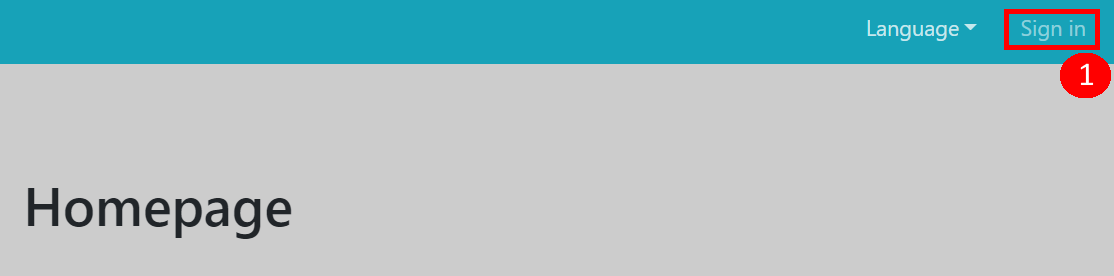
\includegraphics[width=\linewidth]{/userManual/client/login/mainpage}
       	\caption{}
		\label{fig:annoMainPage}	
    \end{subfigure}
    \begin{subfigure}{0.60\linewidth}
        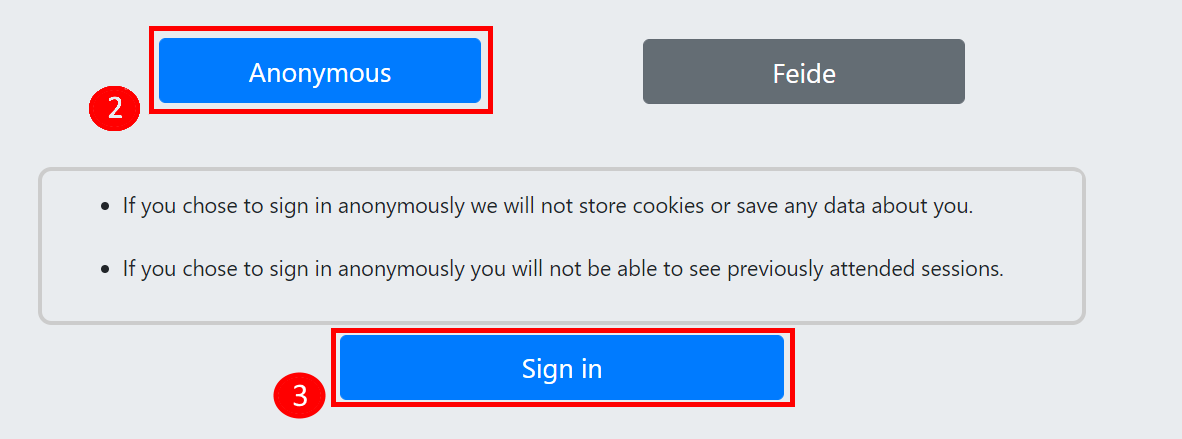
\includegraphics[width=\linewidth]{/userManual/client/login/annoLogin}
      	\caption{}
		\label{fig:annoLogin}	
    \end{subfigure}
    \begin{subfigure}{0.60\linewidth}
    	
\includegraphics[width=\linewidth]{/userManual/client/login/annoResult}
    	\caption{}
    	\label{fig:annoResult}	
    \end{subfigure}
\end{figure}

\begin{userManualItemlist}
	\item[Step I.] Click the Sign in button (1). (Figure: \ref{fig:annoMainPage})
	\item[Step II.] Click the button (2) labeled “Anonymous”. (Figure: \ref{fig:annoLogin})
	\item[Step III.] Click the button (3) labeled “Sign in” to anonymously log in to the page. (Figure: \ref{fig:annoLogin})
	\item[Step IV.] If the login was successful, the navigation bar displays a random animal name. (Figure: \ref{fig:annoResult})
\end{userManualItemlist}

\subsubsection{Feide Login}
\begin{figure}[H]
    \centering
    \begin{subfigure}{0.60\linewidth}
        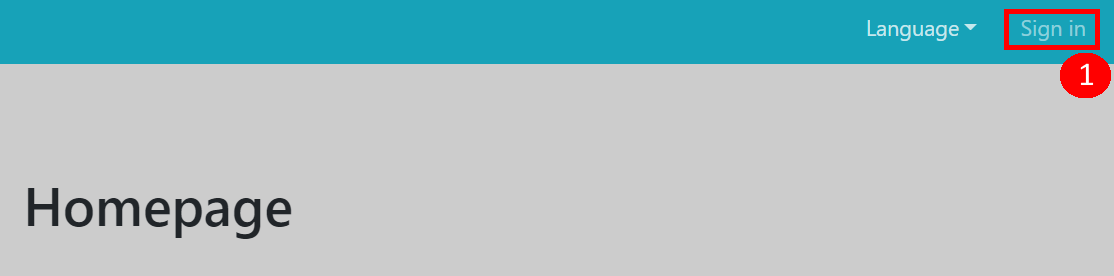
\includegraphics[width=\linewidth]{/userManual/client/login/mainpage}
       	\caption{}
		\label{fig:feideMainPage}	
    \end{subfigure}
    \begin{subfigure}{0.60\linewidth}
        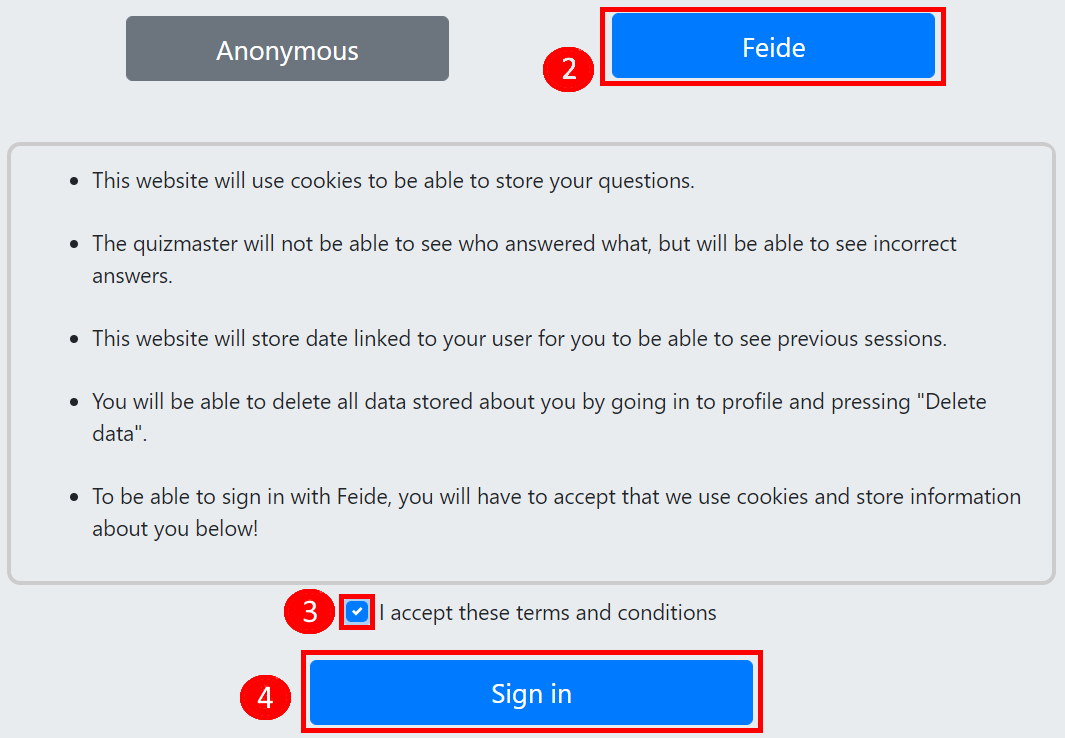
\includegraphics[width=\linewidth]{/userManual/client/login/feideLogin}
      	\caption{}
		\label{fig:feideLogin}	
    \end{subfigure}
     \begin{subfigure}{0.60\linewidth}
        
\includegraphics[width=\linewidth]{/userManual/client/login/feideResult}
      	\caption{}
		\label{fig:feideResult}	
    \end{subfigure}
\end{figure}

\begin{userManualItemlist}
	\item[Step I.] Click the Sign in button (1). (Figure: \ref{fig:feideMainPage})
	\item[Step II.] Click the button (2) labeled “Feide”. (Figure: \ref{fig:feideLogin})
	\item[Step III.] Read through the terms of use!  
	\item[Step IV.] Click the radio button (3). (Figure: \ref{fig:feideLogin})
	\item[Step V.] Click the button (4) labeled “Sign in”. (Figure: \ref{fig:feideLogin}) 
	\item[Step VI.] Follow the instructions given and log in to your Feide account.
	\item[Step VII.] If the login was successful, the navigation bar displays your Feide name. (Figure: \ref{fig:feideResult})
\end{userManualItemlist}


\subsection{Sorting}
Short description about sorting algorithms.

\subsubsection{Insertion Sort}
Insertion sort is simplest sorting algorithm learned in the algorithms and data structures course. Insertion sort uses an easy algorithm that is forced to go though every entry in a list. The algorithm checks whether or not the current entry has a smaller value then the previous entry, if entry has a smaller value, then the previous entries have to re-sorted with the entry until either you find an entry that is smaller or reach the start of the list. 
\\[11pt]
The insertion sort is quite easy to implement, essentially only consists of a for-loop and a while-loop. Because its simple design its a sorting algorithm that is quite often used. Insertion sort is however quite slow compared to most other sorting algorithms. It only has an O(n) average run time, and a runtime of O($n^2$) in terms of worst case scenario.
\\[11pt]
Although insertion sort is quite effective when it is used to sort almost fully sorted list's. This means that insertion sort algorithm is used by a lot of other sorting algorithms. Mostly used as a final step in these other sorting algorithms. Examples of this being the sorting algorithms Shell sort, Merge sort and Quick sort.	%Probably have should have a cite to the different sorting algorithms mentioned just now.

\subsection{Shell Sort}
Shell sort is a sorting algorithm that is based on insertion sort. The key difference between the two sorting algorithms is in performance. Shell sort will have both an average case and a worst case of O(n) runtime. The main reason for this is that shell sort will sort entries in the list that are at certain intervals from each other. The algorithm is essentially dividing list entries into smaller sublists in order to make the sorting more efficient. Through this method, shell sort avoids having to check every entry in the list, which allows the algorithm to remove the main drawback of using insertion sort.
\\[11pt]
The starting interval used in a shell sort is usually based on approximately half length of the list. The algorithm uses the interval to divide up the entries in the list. The entries chosen together are then compared to each other and sorted based on their value. Once the list has been effectively sorted on the current k-interval, the interval's value is halved and the sorting process starts anew. Eventually, the interval will reach a value of 1, which causes shell sort to finish sorting the list using the insertion sort algorithm. Of course, since the list should at this point be almost completely sorted, and therefore the insertion sort should never achieve a run-time of $O(n^2)$.

\subsubsection{Merge Sort}
While performing the sort, every stage of the algorithm is saved in a list of steps. There are three stages which are stored as a step.
\begin{itemize}
    \item Initial. The initial step is stored before the sorting starts. It contains a copy of the unsorted array and a reference to the limit.
    \item Split. The split step is added when an array is split into two arrays. It contains a copy of the array being split, and copies of the new arrays.
    \item Merge. The merge step is added after two arrays have been merged to a new array containing the sorted version of all the elements. It contains a copy of the two arrays being merged and a copy of the resulting array.
\end{itemize}
When implementing the algorithm, performance and memory usage were not considered to be important. The algorithm runs only once per question to generate the steps so that each student's answer can be compared to the right way of performing a merge sort. For this reason, the intermediate arrays are allocated dynamically instead of being reused in later steps. This gives the algorithm worse performance, but its average case performance is still $O(n * logn)$. Memory usage has not been considered because the algorithm has to store more information than normal to store the steps.

\subsubsection{Quick Sort}
While performing the sort the algoritm we wrote also stores the state of steps that we picked. This is done for the solution checker to be able to check if the student has drawn the correct answer when simulating the quicksort algorithm.
\begin{itemize}
    \item Initial: The initial step is stored before the sorting starts. It contains a copy of the unsorted array.
    \item Split: The split step is stored each time the algorithm splits a list, it will store the unsorted list that it will split, the pivot point, left and right list.
    \item Merge: The merge step is stored each time the algorithm merges the sorted lists and pivot point. It will store information about the sorted left and right list, the pivot point and the sorted list after the merge.
\end{itemize}
\begin{figure}[H]
    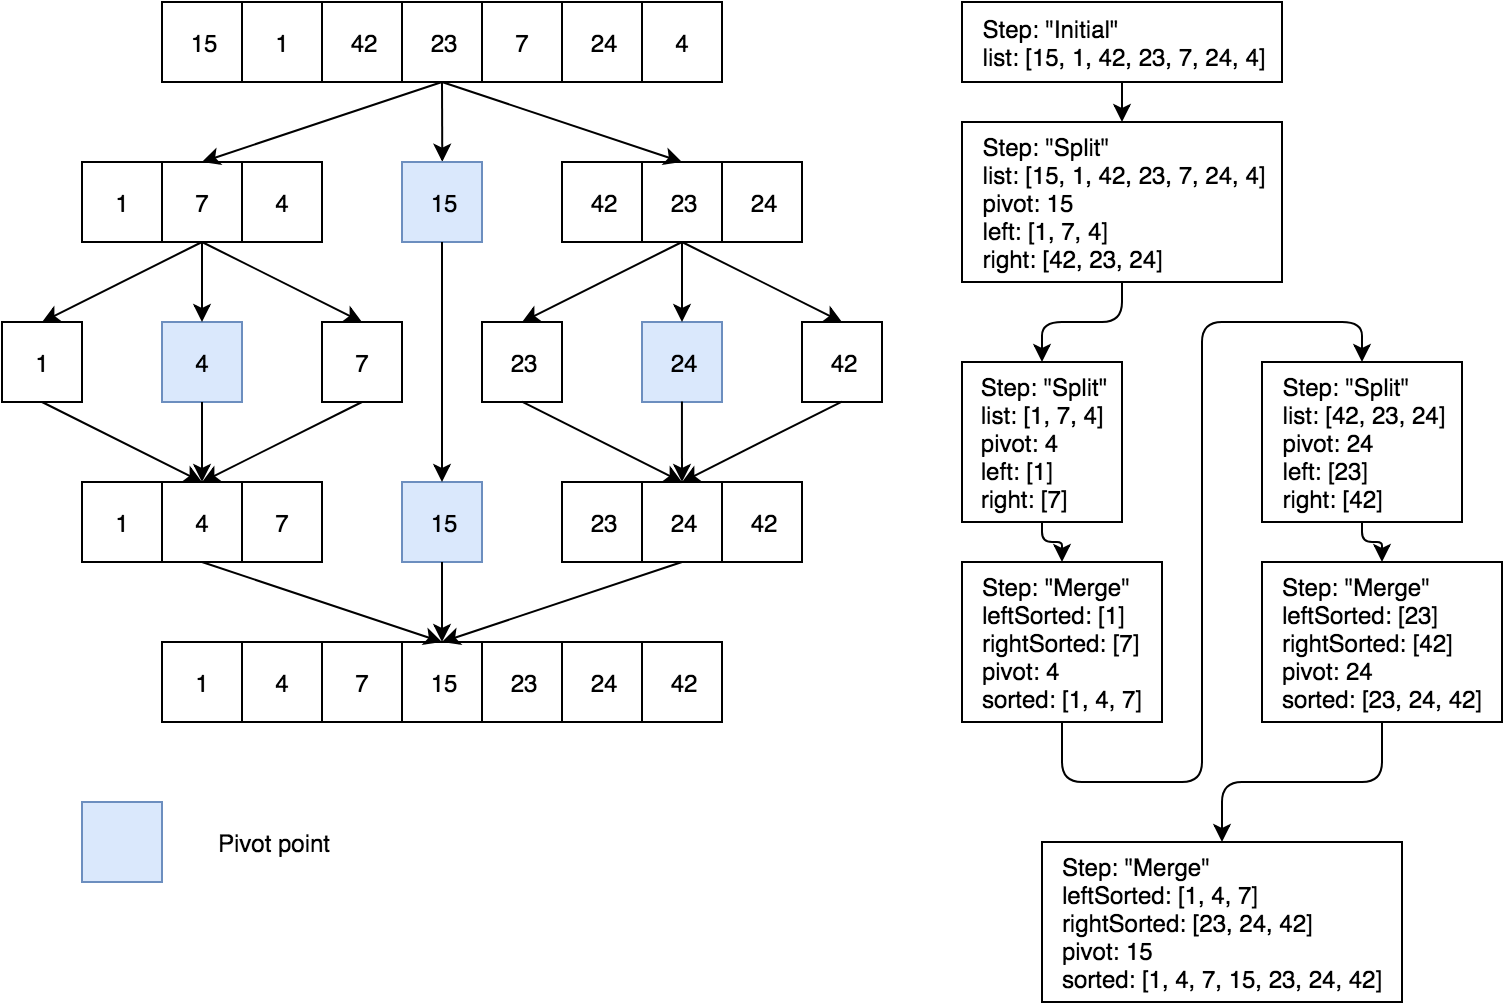
\includegraphics[width=\linewidth]{/diagrammer/Quicksort}
    \caption{Quicksort}
    \label{fig:quicksort}
\end{figure}


\subsection{Data Structure}
%Insert boring text here
\subsubsection{BinaryTree}
A binary tree data structure is a simple data structure whose structure resembles a tree. A binary tree consists of nodes each having an unique value. Each node has a reference to its parent node and its children nodes. The previous node that links to the current node is called a parent node. The child nodes are the next nodes in line after the current selected node. A tree node can only have up to 2 children node, and every node must have only 1 parent node. The exception to this rule is the very first node in the tree, which is called the root node. There can only be 1 root node in the tree. Since a node can only have up to 2 children nodes, the child nodes are usually referred to as either the left child node or the right child node. A node that has no child nodes will always be at the bottom of the tree, and are referred as leaf nodes. The binary tree data structure is notably used as file systems. 
\\[11pt]
Most of the student tasks involving binary tree, usually involves drawing a resulting binary tree. In order to avoid giving the students help with drawing a correct binary tree structure, the graph drawer was designed in a way that lets them mix between drawing tree structures and graph structures. However, this essentially meant that multiple extra criterias  needed to be considered when checking the students work with the solution. It was necessary to implement a Javascript class Tree for representing the binary trees drawn and a Binary Node class representing every node in the tree. These classes were designed in a way that they could be used in all the taught binary tree structured in the Algorithms and Data Structures course. This being the normal binary tree structures, binary search tree structures and AVL binary tree structures. 
\\[11pt]
The Tree class consists of a root node referencing the node at the start of the tree, and an array of all the current nodes in the tree, this also includes the root node. The Binary Node class consists of the node's value and an array containing the node's child nodes. A notable design choice chosen was that each binary node and all their children nodes are stored in arrays. The tree has an array of all current nodes in the tree, where index 0 will be the root node. In addition all nodes have an array containing references to its children nodes. Normally a tree structured would have only needed having an independent variable referencing the two different child nodes, however because students could essentially draw any kind of tree, it was a better option to store the children references in arrays instead. The reason this was because a student had the option to draw a tree with more than 2 children, which is not allowed in a binary tree structure. Arrays also doesn't cause any problems with distinguishing the different child nodes either since the nodes will be divided properly using different placement indexes. Left child will always be located at index 0 and the right child node will always be located at index 1. If there are more than 2 children nodes in the array, then the binary tree criterias are not fulfilled, and therefore will not be accepted as a valid tree object. Multiple functions were implemented to not only transform the drawn tree to a Javascript tree object, but also to check whether or not the created Javascript object is qualified as the chosen binary tree structure. Additional inbuilt class functions for both the tree class and node class were needed for certain tree interactions. For instance, in order to avoid problems with overwriting old tree structures when the program required a new tree with the same property as the old was needed, a duplicate tree function was added to the tree class.


\subsubsection{BinarySearchTree}
The solution checker is designed to check that the tree object created from the students drawing, matches the tree created in the solution. The solution checker recursively calls a function named \code{checkNode} that compares each node in the tree with the corresponding node in the solution. If the two nodes do not match, the solution checker returns false, and the student has answered incorrectly. If all nodes compared match the solution, the solution checker returns true, meaning that the student has answered the question correctly. The solution checker traverses the tree inorder. It will first check the left node, then the parent, then the right node. This solution checker is also used for AVL trees.
\\[11pt]
A function \code{createBinarySearchTreeSolution} was implemented to create a BST based on given arguments and/or existing tree object. This function was implemented so that the admin did not need to manually create the solution trees for each question. The function takes an array with integers and possibly an existing tree as parameters. If the existing tree is not given, the function creates a new tree based on the values in the array. If an existing tree is given, the values in the array are added to this tree instead. It is important to note that the function will not work with duplicate values in the array or given tree.
\\[11pt]
The \code{createBinarySearchTreeSolution} also needed to create resulting trees upon deleting an existing node in a tree. Because there are multiple ways to choose nodes for replacements when deleting a node with two children. It was required for the \code{createBinarySearchTreeSolution} to create a list of the potential final resulting trees. It is required to specify whether the user wants to add nodes or remove nodes from the tree when creating the solution trees. The function cannot switch between the two during execution, and an existing tree is required in order to remove nodes in the tree.
\\[11pt]
The \code{createBinarySearchTreeSolution} returns an array containing the different states of the BST during its creation. Since there can be different resulting trees when deleting a parent node, all resulting trees are stored in an array. The last element in the array is the finished BST tree object that is compared with the drawn tree from the students. Originally the drawn tree from the student is a graph object and has to be transformed into a \code{Tree} class object using the general tree function \code{createTreeObjectFromCanvasObjectver1}.Once transformed into a BST object the student tree is compared with all the trees in the solution object in the solution checker.
\begin{figure}[H]
    \centering
    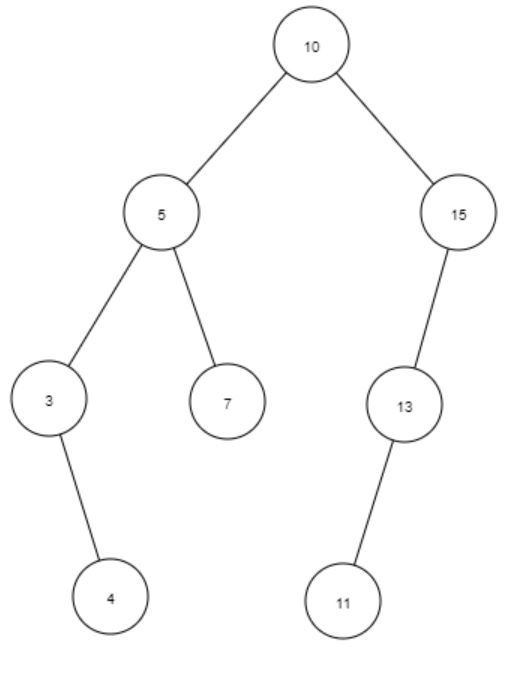
\includegraphics[width=250px, height=250px]{/trees/BST}
    \caption{The figure shows an example of a Binary Search Tree.}    
    \label{fig:BST}
\end{figure}

\subsubsection{AVL}
\begin{figure}[H]
    \centering
    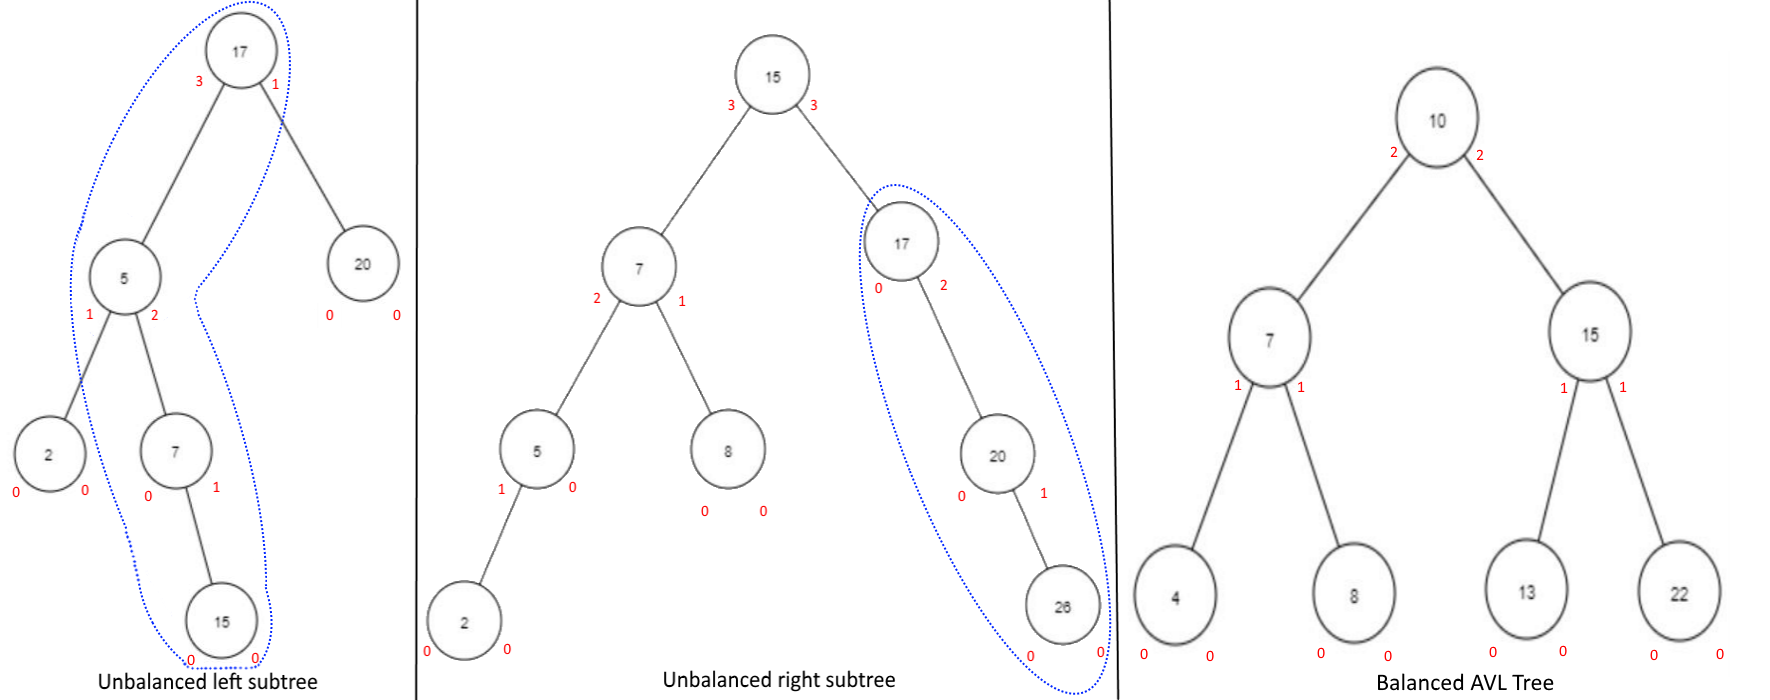
\includegraphics[width=0.90\linewidth]{/trees/AVLTreesVer2}    
    \caption{The figure displays 2 unbalanced binary search trees and a fully balanced AVL tree. }
    \label{fig:AVLTrees}
\end{figure}
\noindent
An example of balanced and unbalanced BSTs can be seen in figure \ref{fig:AVLTrees}. The left tree is a BST that has too many nodes in the left subtree. The center tree is a BST that has too many nodes in the right subtree. The tree to the right in the figure is a fully balanced BST, which makes it qualified as an AVL tree. The red letters represent the height of the node's children. The value is determined by how many nodes there are between the leaf nodes to the selected node. The blue dotted lines mark the subtree that breaks the AVL condition.
\\[11pt]
In this project, the name of the rotation direction is based on which subtree side has the most nodes. This means that in the previous example\ref{fig:AVLTrees}, the middle tree, a right rotation was needed that would have rotated the right subtree one step to the left. The opposite happens in a left rotation; too many nodes in the left subtree will make it rotate in the right direction. In some circumstances, a double rotation is needed. These, on the other hand, are named after the last direction the nodes need to rotate in order to balance the subtree. Double left rotation means that a rotation towards the right is first used on the right child of the node causing the imbalance. This switches the right child's spot with the imbalanced node. Then followed by a rotation on the new imbalanced node towards the left. The opposite will occur on a double right rotation.
\\[11pt]
The function \code{createAVLTreeSolution} creates an AVL tree used as the solution object for a question. The functionality is mostly the same as the \code{createBinarySearchSolution} function mentioned earlier. However, some extra functionality was needed in order to balance the tree. If an existing tree is given, the given tree needs to be fully balanced before any insertions or deletions can be done to the tree. Once the existing tree is balanced or no existing tree was given, the values in the added array are inserted in the tree. Just like in \code{createBinarySearchSolution}, removing nodes from a tree requires that an existing tree is given. After every insertion and deletion, the tree will once again have to be checked to see whether or not it is still balanced. If the tree is not balanced, the tree will have to rotate in order to rebalance itself. The rotation is determined by which subtree currently has the most nodes. Not to mention insertion and deletion require a different set up when it comes to using normal rotation or double rotations. The returning array from the \code{createAVLTreeSolution} is used and has the same format as in the \code{createBinarySearchSolution} function. The only noticeable difference is that the array for the \code{createAVLTreeSolution} also need to store the tree state after any rotations have been performed.
\\[11pt]
Because the \code{Tree} class contained circular references between a parent node and child nodes, it proved difficult to store solution BSTs and AVL trees into the database. This was because it was not possible to convert the tree object to JSON, since JSON cannot handle circular references. This means that the circular references had to be removed before the solution could be stored in the database. To solve this an export function was implemented for the \code{Tree} class. The export function removes the circular references by turning the parent reference into the parent's node value. Once the parent reference is gone, the tree object was able to be converted to JSON format. Of course, since the solution checker requires BSTs and AVL trees to be in a certain format, an import function also needed to be used to convert the tree object back to its original form. The import function has two tasks. The first task is to replace all null values with an undefined value. The second job is to reinsert the proper parent reference to each node in the tree. This is simply done by traversing the tree and remembering the previously visited node as the current node's parent. Once this is done the solution object can be checked with the converted tree the students drew with the GraphDrawer and see if they match or not. If the question revolved around removing nodes, then the converted tree only needs to match one of the trees in the solution object.



\subsection{Algorithms}
\subsubsection{Dijkstra}
\subsubsection{Bellmanford}
\subsubsection{BFS}

\subsubsection{GraphDrawer}
If new question types are implemented which require the GraphDrawer to keep track of thousands of nodes at the same time, there might be performance issues on some systems. The nodes are currently stored in an array. This means that if the array is searched for a node on the screen, all of the nodes need to be checked, even those on the opposite side of the world. Many operations starting on one node, and ending at a node close to the first node (e.g., selecting nodes by dragging the mouse) would be more performant if a spatial data structure\cite{SpatialDatastructure} was used instead.
\\[11pt]
The current system is designed to work with both touch screens and cursors. Because of this, two choices were made to make the development simpler and less time-consuming.
\begin{enumerate}
    \item When a user needs to enter text or numbers, the JavaScript alert popup is used because this works in all browsers. Some users with a keyboard would have been able to write faster if the GraphDrawer read the input directly. Mobile browsers do not allow a website to open the virtual keyboard from a script. If the mobile browsers change this in the future, a different method for retrieving the user input could be used. Some browsers allow the user to block popups. If this is done, the user can no longer enter text.
    \item For simplicity both desktop and mobile users control the GraphDrawer the same way. User testing can be done to find the gestures which feel the most natural. If the natural way to do something is different depending on the system, different handlers can be implemented.
\end{enumerate}
Every time the world state changes, the canvas is redrawn. Changes outside the camera view should not make the GraphDrawer redraw the world. If only a small part of the world inside the camera view is changed, only that part needs to be redrawn. This has not been implemented because there have not been any performance issues with the current question types.

\subsection{Python}
Python is the programming language used in the DAT100 course at UiS. Students are often struggeling to understand the difference between value type and reference type variables. To make it easier for them to learn, a Python interpreter was implemented which evaluates Python code step by step. Together with the GraphDrawer, the interpreter can be used to ask questions about Python code. The student is able to see whether a variable is value or reference type, and they can see when the value or reference changes. Before implementing a custom interpreter, using the offical Python interpreter was considered. Because of the size of CPython, and the limited time available for this project, it was decided that implementing a custom interpreter was the better option.
\\[11pt]
The following features of Python are supported:
\begin{enumerate}
    \item Variables of the following types: Number, String, Boolean, and Object.
    \item Functions can be defined using the \code{def} keyword. They can either belong to the global scope, or to a class. Functions can return something using the \code{return} keyword.
    \item Classes can be defined using the \code{class} keyword. If a function with the \code{__init__} is defined inside the class, it will be called when a new instance of the class is instantiated.
    \item If statements can be used with the \code{if} keyword. Elif and else statements are also supported.
    \item The following mathematical operators are supported: +, -, /, *.
    \item The following comparison operators are supported: and, or, !, ==, !=, <, >, >=, <=.
    \item Expressions can be grouped and seperated using parenthesis.
    \item Lines starting with a # are treated as comments, and will be skipped by the interpreter.
\end{enumerate}
Significant Python features missing from this interpreter:
\begin{enumerate}
    \item The standard library.
    \item Lists and dictionaries.
    \item Inner classes and functions.
    \item Shared class variables.
    \item Class inheritance.
    \item Loops.
\end{enumerate}
Every operator has the same priority, which means that expressions are always evaluated left to right. This makes some expressions not behave like expected. The following statement results in an error: \code{if 1 + 1 == 2:}, because it is evaluated as \code{1 + (1 == 2)}. To prevent this from happening, parenthesis should be used to order the expressions. The correct statement would be: \code{if (1 + 1) == 2:}.

\subsubsection{Interpreter}
There are three main functions in the interpreter. \code{parseLine} which tries to figure out what the meaning of a code line is. \code{parseLine} is also responsible for deciding which line to parse next. A line can either be a variable assignment which is handled  by the \code{parseLine} function, an expression which is handled by the \code{evaluateExpression} function, or a statement which is handled by the \code{handleKeyword} function. A statement is anything which starts with one of the keywords. An expression is something which can be evaluated to a value.
!! Insert fancy image showing the path code goes trough the interpreter !!
\\[11pt]
An important feature of the interpreter is the scope objects. A scope is an object which stores information about the variables, classes, functions and data inside the scope. Functions are scopes because they can contain private variables. Classes are also scopes, because they can contain functions. Before code can be parsed, a global scope is created. Anything which doesn't belong to a specific scope, is placed in the global scope. Scope data is an array where the index is the address of the stored data, and the value is the stored data. Because the interpreter is implemented in JavaScript, there is no need to seperate value and references types in this array because JavaScript and Python behave the same way. Scope variables are a mapping from variable names to data addresses. Scope functions/classes are mappings from function/class names to function/class objects. Because the interpreter should save the state of the program as steps, the \code{parseLine} function returns an object containing information about the state. If the state was anything other than a function or class definition, the current state is saved as a step.
\\[11pt]
A function is an object with a \code{name}, a list of arguments \code{args}, a list of the code lines belonging to the function \code{code}. A function should also be a scope. The name is used to identify the function. The arguments are used to make sure that when the function is called, the right amount of arguments are passed. The code is stored so the function can be evaluated when it is called. After a function has been defined, the \code{handleKeyword} function returns a state of type \code{"SkipLines"} which tells the caller which lines have already been handled. The interpreter uses the \code{callFunc} function to call Python functions. When a function is called, three things happen in the following order:
\begin{enumerate}
    \item The function arguments are added as local variables. Local variables mean they belong to the function scope. The arguments need to be in the same order as they were defined, because named arguments are not implemented.
    \item Every line found in the functions \code{code} list is parsed using \code{parseLine}. If a \code{return} statement is found before reaching the end, the function will stop parsing, before reaching the end.
    \item The scope of the function is restored to an empty state and data is returned if a return statement was found.
\end{enumerate}
\\[11pt]
A class is an object with a \code{name} and a list of the code lines belonging to the class \code{code}. A class should also be a scope. When a class is defined, the code is also parsed using the \code{parseLine} function. This is done so that any functions within the class is defined in the scope of the class. When the interpreter is instantiating an instance of the class, the \code{instantiateClass} function is called. \code{instantiateClass} will first create a new object which contains all the functions from the class. If the class has a constructor it is called. Finally, the object is returned to the called of \code{instantiateClass}.
!! Write about expression evaluation !!
!! Write about operators !!

\subsubsection{Questions}
!! TODO: Write this :=) !!

\subsection{Vue}
How the application is set up.

\subsection{Database}
Since the web application requires a database to store information about users, questions, sessions, courses and more, a set of files were created to get, insert and update the information. The database is designed around features needed for the application. It was also created for scalability in mind with for example the possibility to add other OAuth/OpenID connect possibilities in the future. There are five scripts associated with the database, where get, insert and update functions have been separated into their own scripts. One script is connecting the get, insert and update scripts making it easier to import and use the database functions in other scripts. There is also a script which will run every time the server starts. This script makes sure that every table is created and have the correct column names. It is also the script that inserts default values such as question types and the anonymous user.
\begin{figure}[H]
    \centering
    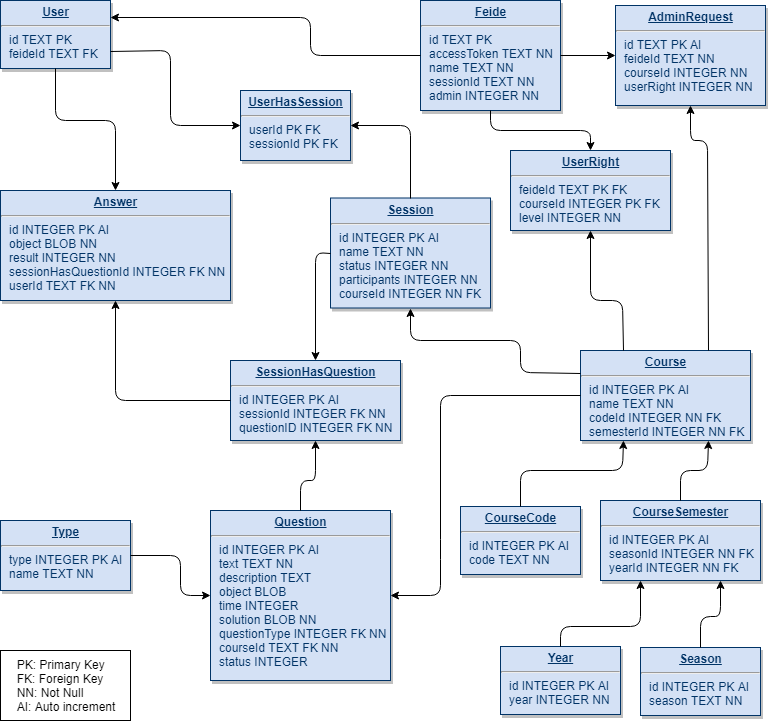
\includegraphics[width=\linewidth]{diagrammer/databaseSchema.png}
    \caption{This is the database schema used for Interaktiv Undervisning}
    \label{fig:dbSchema}
\end{figure}
The table "User" has the anonymous user with user id 1. When an anonymous user answers a question, the answer is linked to that user, no matter who answered. Feide information is in its own table, this makes it easy to add more types of login services, e.g., Facebook, Google, and more. When an admin adds a question to a session, it is linked in its own table called "QuestionHasSession". This is to ensure that a question can be linked to more than one session or multiple times in the same session. The answers are also linked to the "QuestionHasSession" table, making sure that the answers shown to admins are only for that question in that session and not the total answers statistics for the question in general. Sessions are linked to a course. A course contains information about the course code and semester, enabling the option to separate sessions from each semester. Questions are linked to the course id, but admins do have the option to copy questions from one course to another in the question dashboard.

\section{Application}
%Write and introduction to this part.

\subsection{Creating Questions}
Everything in the application that is restricted to admin will only use the Admin.vue component as the view file. In order to start creating questions, the user first need to load the Questions.vue component onto the Admin.vue component. This will call the \$route function in Admin.vue that will you use the vue router to update the path to /admin/questions. This will in return make the Admin.vue load the needed Questions.vue component. The Questions.vue component consist of other components such as EditQuestion.vue, ShowQuestion.vue, SelectCourse.vue and AddQuestionToSession.vue. All components that is related to creating a question can be found in the App/client/components/admin/question folder. On the /admin/questions page there will be a select form to the left, which is in the SelectCourse component. In this select form the user can choose between the available courses in the database. Keep in mind that a course must be chosen for the user to able to create new question. This is done so that a question can immediately be assigned to the given course, since every question should be assigned to at least a course before the question can be allowed to be used in an active session.  If the user attempts to create a question without having a course in the database, an error message will be displayed to the user instead.\\[11pt]
The area in the middle of the Questions component is where the current questions for the selected course is going to be listed. This area has a white background color in contrast with the normal grey background color in order to make it more to noticeable to the user. If there are no questions for the selected course, then this area contains the message “no question.” instead. The Question sends an emit request to the server whenever the component is loaded, the course changes, a question is edited, or a question is created. This emit message will ask server for all the current questions for the current selected course. The server then calls the appropriate select statement in the database and returns the result. The result is then used by the Questions component to update the list of questions. In this way the list should always be up to date with the contents in the database. 
\begin{figure}[H]
	\centering
	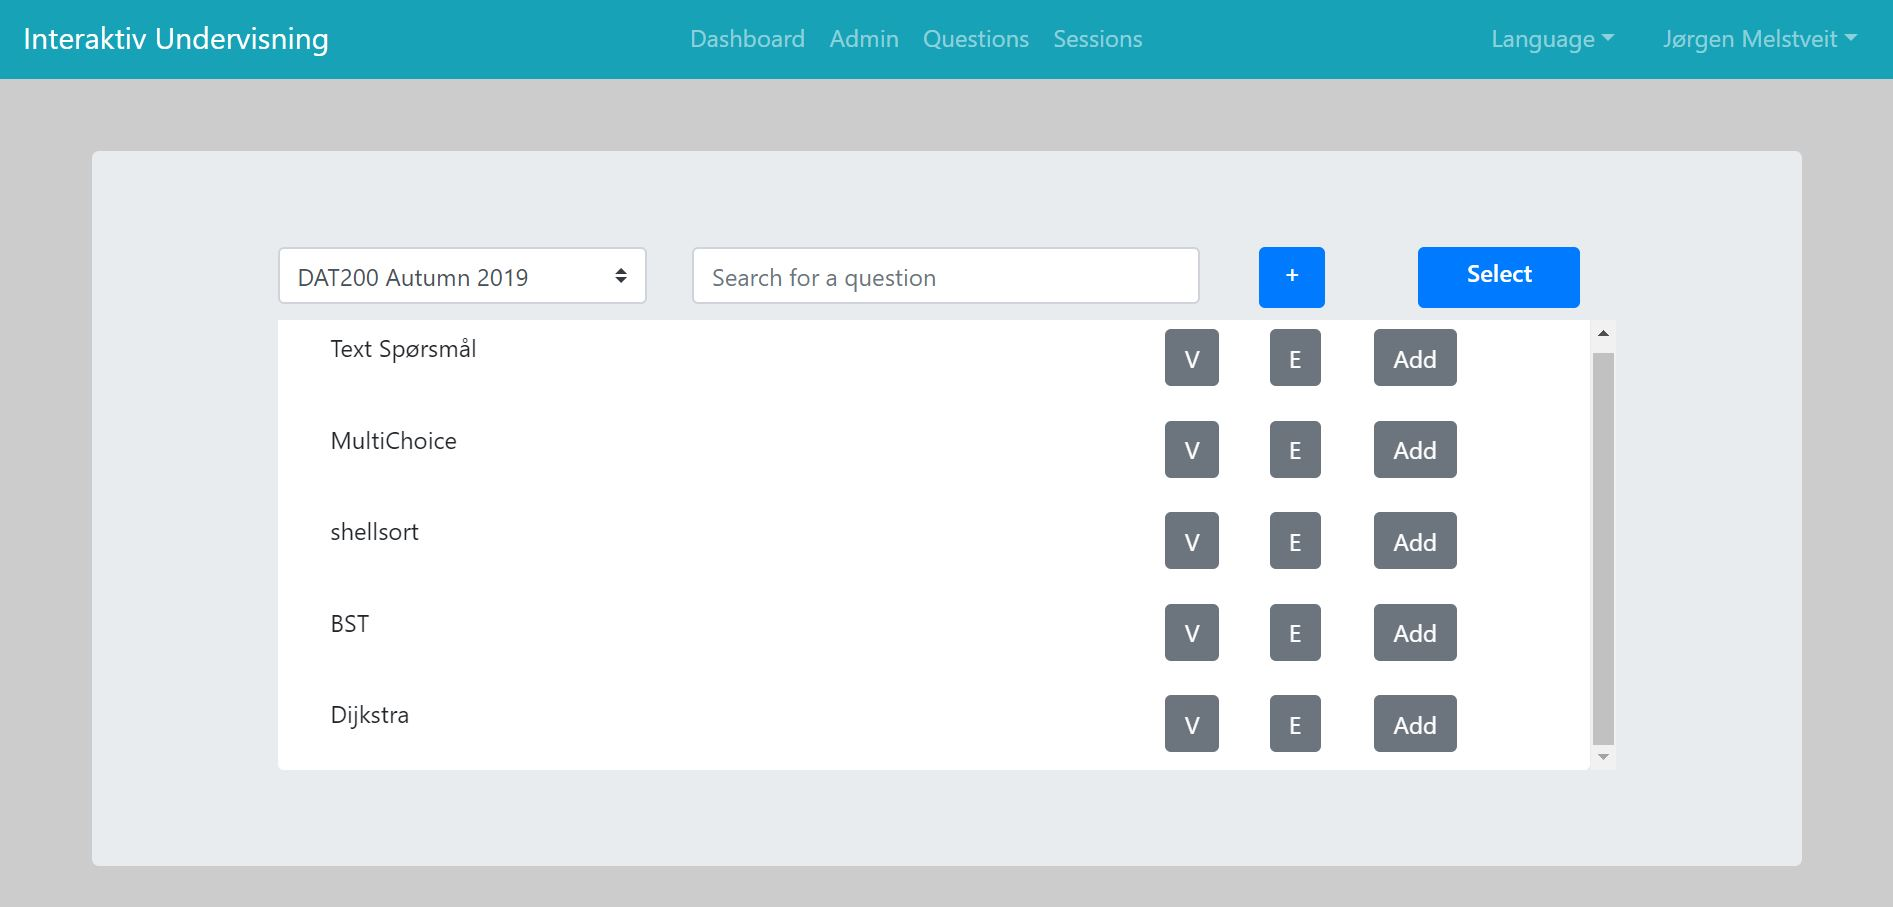
\includegraphics[width=0.80\linewidth]{/createQuestion/questionvueEnglish}
	\caption{The figure displays an image of the Questions.vue. This is the component is primarly used for allowing users to create new questions for a selected course. }
	\label{fig:questionVue}
\end{figure}
\noindent
To create a new question the user first needs to click the button with the label “+”. This will reveal the EditQuestion component which contain a vue-modal element that has all the needed forms needed for creating a question. EditQuestion is a component that is used for both adding new questions and editing existing questions. The main differences between the add and edit operations for the component are the following:
\begin{itemize}
\item[-] The title of the modal will be different. Either its going to be “New Question” for the add functionality or “Change Question” for the edit functionality.
\item[-] The edit functionality needs to load the question data from the database and fill in the forms with the correct information. 
\item[-] The request sent to the server with the question information are different. The server requests are different primarily to distinguish between the insert and update SQL commands used on the database.
\end{itemize} 
Originally there were 2 components used for the two operations, but this was later changed in development because having 2 components that were practically the same was deemed unnecessary. The modal in EditQuestion is divided into 3 parts, namely Basic Information, Media and Solution type.  These parts can be opened and closed to the user’s preference, where basic information is open by default and the other parts will be closed. Basic Information part contains an input field for assigning the question title, a textarea for giving the question a description, a time input field and a time slider. The input field is used for giving the question a title. The textarea and the time slider are both using v-model to mount to the variables newquestion.description and time respectively. These can be found in the intializeState function. This is done so that data in these fields are relatively easy to acquire and keep track of. The time input has a watcher that checks for changes to the variable that the time slider is mounted to. This means that these elements always changing their value dependent on the other, resulting in them having the same value. If the time is set to “00:00”, then the question will not have a timer when used in a session.
\\[11pt]
The media part is an optional part and is not required to be used to make a new question. The “Media” part on the EditQuestion component consists of a select box. The select box is used for choosing the wanted media type. Once the select box has the value “images”, the media part is set up for adding images to the question. This in turn will make a button appear with the text “Choose a file upload...”. This button is used for adding an image to the question. Once the button is clicked the file browser will be displayed for the user and allow them to choose an image on their computer and put it onto their question. Once the image is chosen, the EditQuestion component will take the image and then validate the image given. It is important to check that the file taken was an actual image file. If the validation passes, then the image is turned into a buffer. When the question is going to be saved on the database, the question will also contain the file paths to the images given to the question. The buffer is then sent to the server and is turned back into an image. Now that the buffer is removed the path to the image is stored in the database. Whenever a question is obtained from the database that has images, the server will collect the images by using the routes stored with the question. When the image is going to be used on the client again the image will be transformed back into a buffer. A question cannot have to many images assigned to it, as this would take up a lot of the needed data. The total amount of files attached to a question cannot exceed 1.5MB, and the user will get a warning once the amount exceeds 500KB.
\textbf{INSERT Media info about Tables and Graphs here!}
\\[11pt]
The solution type part focuses on setting the question type to the new question and for creating the questions solution. The type will control what format the question will have for both the solution and for the client during a session. Most of the question types available are usually centered around a data structures or an algorithm from the Dat200 or Dat100 courses. There are also normal question types like multiple choice and text questions. The question type chosen will alter the available options in the solution type, so that the user can fill in the information needed for the chosen algorithm or data structure. For instance, Binary Search, AVL, Python and Dijkstra question types all require the GraphDrawer tool. The solution for questions revolving data structures and algorithms are created on the server in the solution generator. The user only needs to apply the necessary information for the question so that it is possible for the student to solve it, and for the server to be able to create the solution. As stated, before the necessary information needed for the question is determined by the question type. The are 2 reasons for having the server handle the solution. The first reason is to keep it away from clients participating in a session. The second reason is because forcing the user write the entire solution in every question created would be rather tedious for the admin user. Not to mention reducing the chances of having the solution being written incorrectly.
\begin{figure}[H]
	\centering
	\begin{subfigure}{0.70\linewidth}
		\includegraphics[width=\linewidth]{/createQuestion/editQuestionUnopenedEnglish}
		\caption{This figure displays an image of the EditQuestion component when all the 3 parts Basic Information, Media and Solution type are hidden. Clicking on the labels would reveal the content of chosen part.}
		\label{fig:editquestionUnopened}
	\end{subfigure}
	\begin{subfigure}{0.70\linewidth}
		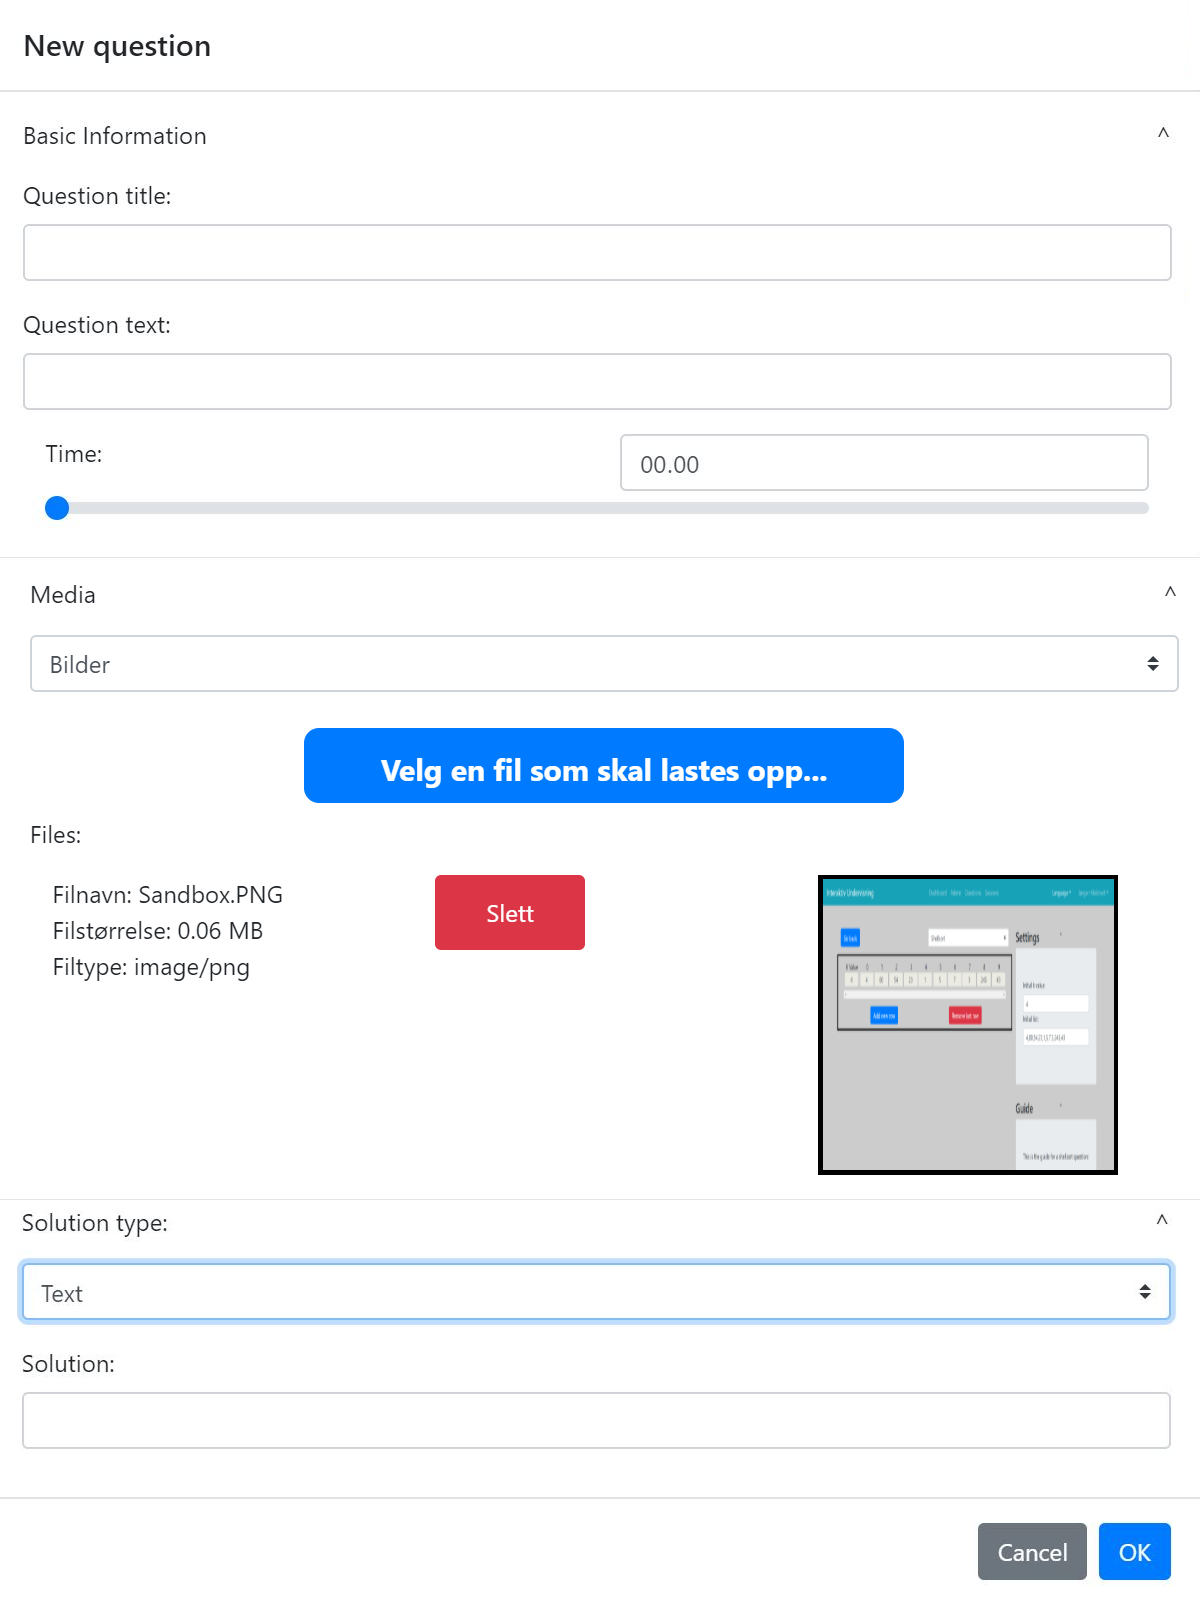
\includegraphics[width=\linewidth]{/createQuestion/editQuestionCombined}
		\caption{This figure displays an image of the EditQuestion component when all the 3 parts Basic Information, Media and Solution type are displayed. Clicking on the labels would hide the content of chosen part.}
		\label{fig:editquestionOpened}
	\end{subfigure}
\end{figure}
\noindent
Once the question is finished the question information will be sent to the server through a socket emit request. The data sent to the server is the newQuestion object found in the function initializeState() in the EditQuestion component. Since all the variables in the newQuestion object are linked to the EditQuestion component, the server should have all the information it needs for the questions solution to be created. However, to avoid any problems regarding storing faulty questions on the server, the question information will first need to be validated by the server's validation checker. The user must at minimum fill in the information in basic information and solution type for the wanted question to be valid. The question information sent to the server will first be validated on the basic information in the question. After that, if the question has an attached media to it then it is validated next. Finally, another validation test that is determined by the given questions type. Pretty much all the question types have their own unique check in the validation checker which are separated in different JavaScript files. If validation checker returns false, then the question failed the validation criteria and the errors given by the validation checker will be returned to the EditQuestion component as an alert box. The errors received by the validation can be vary, but all error message that were triggered will be shown to the user in the alert box. The text shown in the alert box for each error message from the validation checker are stored in the locale files. If the validation succeeds, then the information is sent to the solution generator that generates the appropriate solution in accordance to the questions type.\textbf{INSERT more details about the solution generator}. Once this is done, the question information and solution are inserted into the question table in the database. After the question is stored in the database, the EditQuestion component is closed, and the user is returned to the Questions component. The Questions component is then going to update its question list to accommodate for the changes done on the database.
\\[11pt]
Once a question is created and is listed on the Questions component, there will be more options available for the user regarding the question. The button with the drawing symbol label will open EditQuestion component and let you edit the information previously saved for the question. Do keep in mind that the changes to the existing question are not going to be saved unless a new request is sent to the server. This means that the new question info given must also be fully validated by the validation checker, and a new solution needs to be created for the solution generator to overwrite the previous solution. If the validation fails, then the edits will not be saved in the database. It is also not possible to edit a question type once it has been assigned to a session. Once a question is assigned to a session, it will have its status to change to active. This is indicated on the question on the Questions component when the edit button has a grey background. The reason for not allowing any question to be altered after it has been assigned to a session is because it would affect the saved data after a session is finished. Which means that when a question has been assigned to a session, then that question is deemed finished by the application and can should no longer be altered.
\\[11pt]
The button labelled the eye symbol causes the component ShowQuestion to become visible. This component will load in all the information regarding the chosen question. The ShowQuestion consist of a v-modal that has similar design to the EditQuestion component. Its divided into the same three parts as the EditQuestion, where Media is only shown in the component if any images, tables or graphs are included in the question. In the basic information section, the user can view the basic information of the question like title, description and the time limit. In the media section, the user can view all the images, tables or graphs currently linked to the question. This includes information about the file such as name, type and the size. In the solution section the solution for the question will be displayed. What is shown is dependent on the solution type. Text, Multichoice and Binary tree will show the answer/answers in plain text. Every other question type will use the GraphDrawer tool to display the solution. 
\begin{figure}[H]
	\centering
	\begin{subfigure}{0.80\linewidth}
		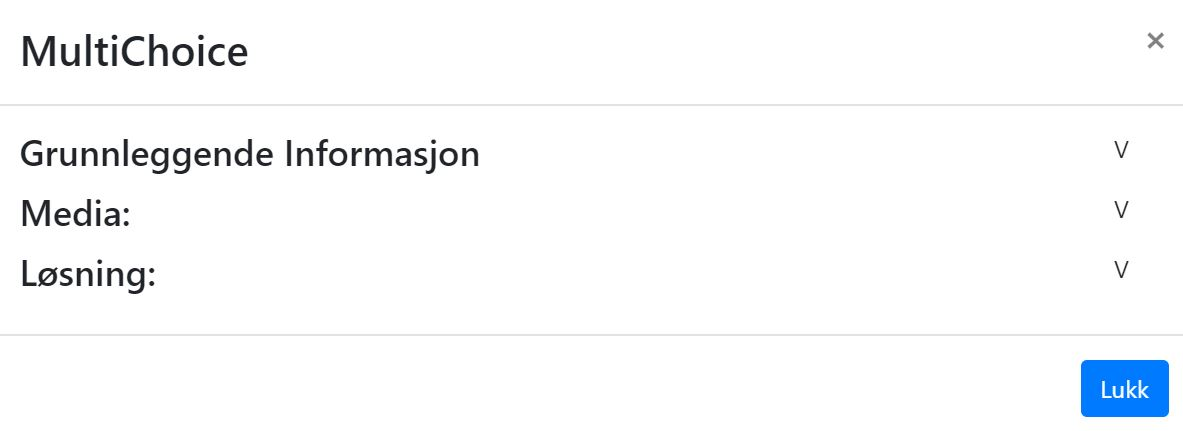
\includegraphics[width=\linewidth]{/createQuestion/showQuestionEnglishUnOpened}
		\caption{This figure displays an image of the ShowQuestion component while all the 3 parts are closed. Clicking on the labels should open op the chosen part.}
		\label{fig:showQuestionUnOpened}
	\end{subfigure}
	\begin{subfigure}{0.32\linewidth}
		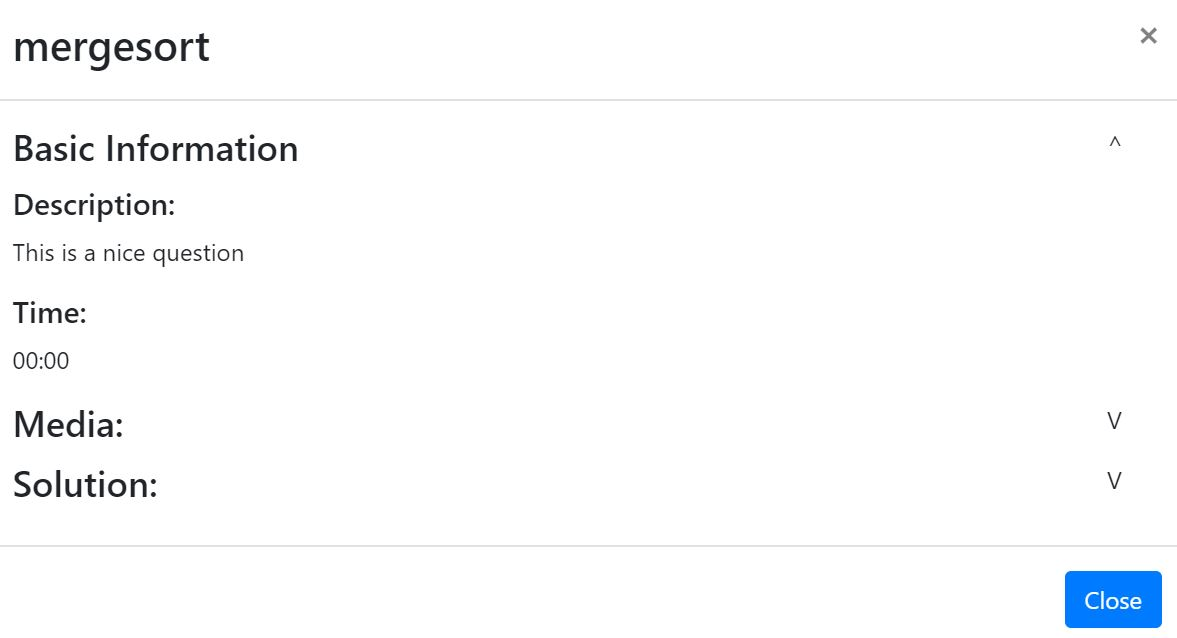
\includegraphics[width=\linewidth]{/createQuestion/showQuestionEnglishBasicOpened}
		\caption{}
		\label{fig:showQuestionBasicOpened}
	\end{subfigure}
	\begin{subfigure}{0.32\linewidth}
		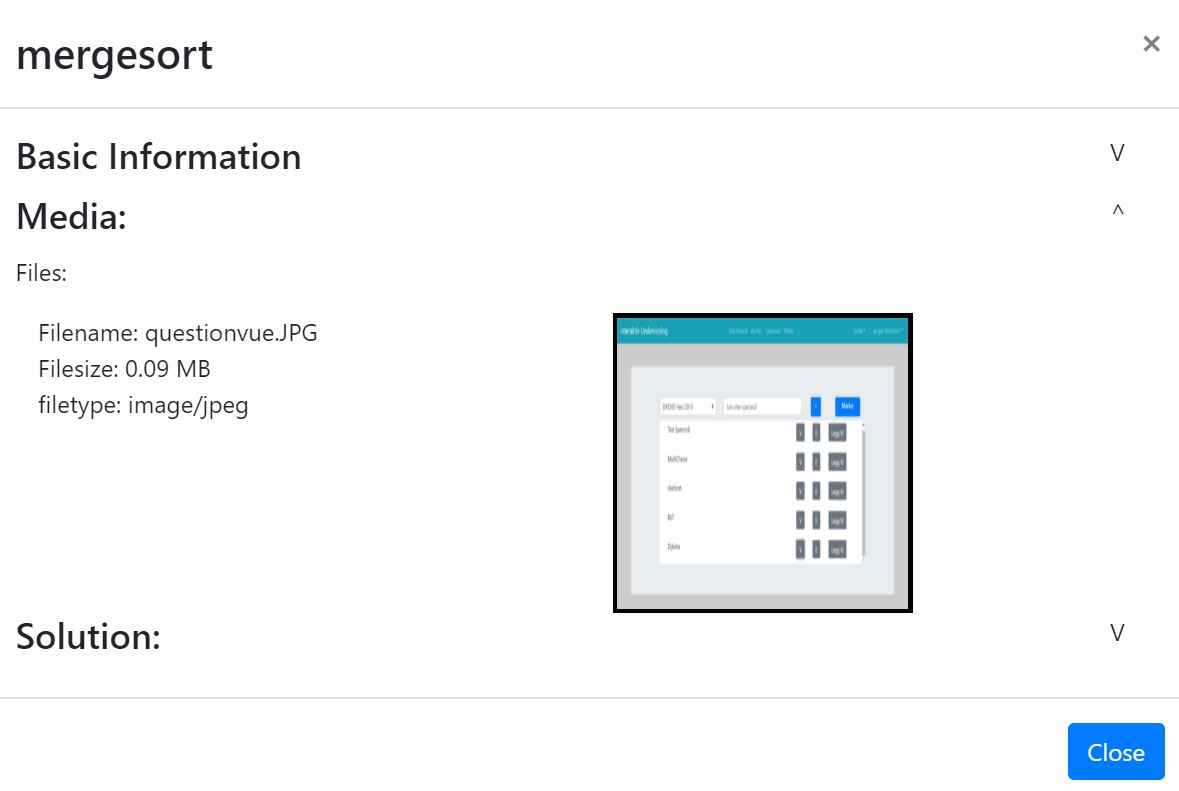
\includegraphics[width=\linewidth]{/createQuestion/showQuestionEnglishMediaOpened}
		\caption{}
		\label{fig:showQuestionMediaOpened}
	\end{subfigure}
	\begin{subfigure}{0.32\linewidth}
		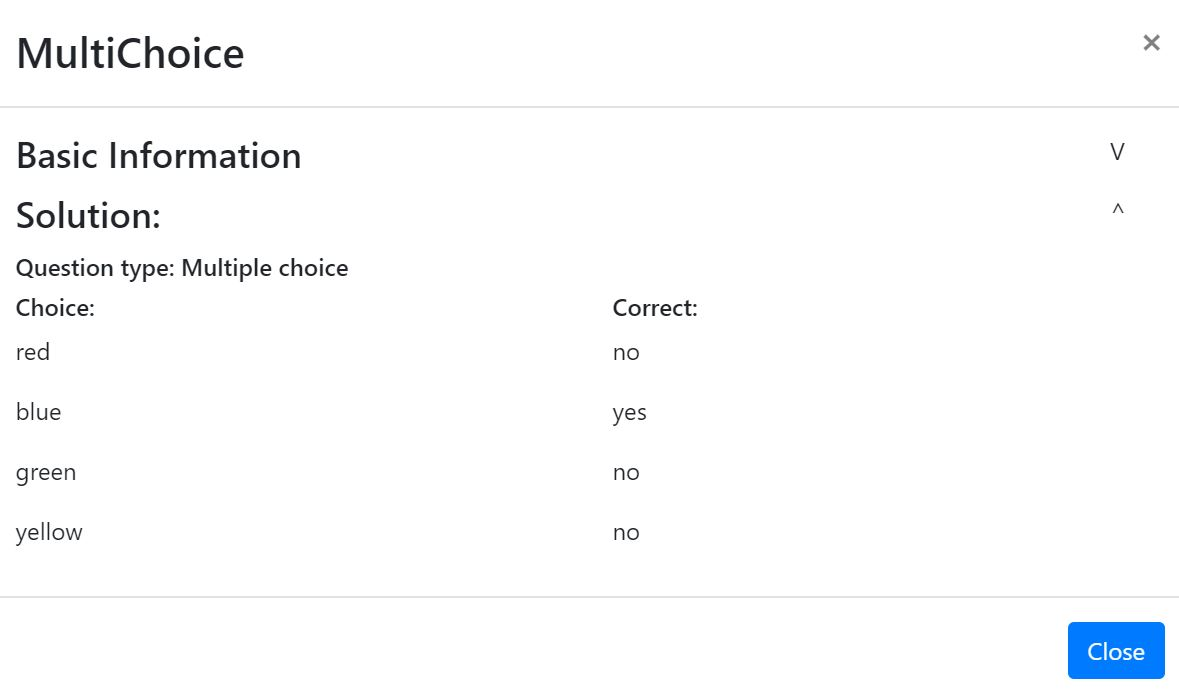
\includegraphics[width=\linewidth]{/createQuestion/showQuestionEnglishSolutionOpened}
		\caption{}
		\label{fig:showQuestionSolutionOpened}
	\end{subfigure}
\end{figure}
\noindent
\textbf{Insert about practical test for questions.}
The last button labelled Add will show the addQuestionToSession component. This component will only display a select box containing all current available sessions in the database. The user can select box one of these sessions and add the chosen question to the chosen session in the select box. This was implemented to give admins the options of adding more questions to an existing session, without having to create an entirely new session just for adding an extra question.
\\[11pt]
Lastly the Questions component allows you to mark question in the list by clicking on the button with the label “Select”. Once the button is used, the user has the option of either copy the selected questions to another course or deleting the questions from the current course. When a question is copied an identical question is created where the course id foreign key is assigned to the chosen course and is stored in the database. When a question is deleted, the question is simply deleted from the database. To exit the select mode simply click on the select button again, which now has the label “Close”. The copy button will use the CopyQuestions component while the delete button will use the DeleteQuestions component. If the user attempts to copy or remove without having selected a question, then an alert box will appear stating that there are no questions currently selected. Keep in mind that it is not possible to remove questions from a course if its already been used in a session. The reason for this is that the question information is still needed for Feide users to look at their previous participated sessions. If the question were to be removed after having been used in a session, then the student wouldn't have access to the question information. Therefore, the students would have no way of looking at their old session results. 
\\[11pt]
The question structure for this application was specifically chosen in a way it would be easier for developers to implement and add new questions types. Excluding the work that is needed for writing the actual data structure or algorithm and its solution format, all that is required in order for a new question type to be added to a session is the following. Create a vue component in both the questionResultScreenAnswer and questionResultScreenSolution directories. These are going to be used for DisplayQuestion component which is used for showing session results after each question. Next add a b-form-group to the EditQuestion component where only the necessary form items and Graphdrawer are set so that the user can create the new question type. If the question type requires a certain unique information, then an extra variable in the newQuestion.objects in the initializeState function should also be assigned and modeled appropriately to the html element in the form group. Then add a JavaScript file in the validation checker for stopping illegal actions to the new type. Then implement the solution generator for the question type which is going to create the format for the solution object stored in the database. Finally create a solution checker that is going to verify that the student answered the question correctly according to the solution object that was withdrawn from the database. The user may also have to update the locale files as well if some new predefined text is needed.\\[11pt]




		
		% Evaluation
		\section{Evaluation}
\subsection{Vue}
To make the interface between the code and the website simpler, we wanted to use a web framework. We needed a dynamic webpage where the different parts were constantly changing depending on the user interaction. Code separation was important for us because we wanted to be able to split it up as much as possible to minify the risk of one error affecting the entire application. We expected Vue to make this easier. Code reuse was also important. We knew from the beginning that the questions and solutions were going to be displayed on different pages, and we wanted only to write the code for this once. We had previously used templating engines, which makes it possible to use JavaScript variables directly in the HTML. This is something we expected Vue to do for us.
\\[11pt]
We had no experience in making single page applications, so we had a lot to learn. Vue met our expectations, and also had many features we did not know about. Examples are the Vue Router. We did not consider the fact that when there is only one page, the user cannot use the URL bar of the browser to navigate. We had some problems with storing application state between different views and components, but after some searching, we found Vuex which was made to solve that problem. Our experience is that Vue did not prevent us from doing anything we wanted to do, and it provided good solutions to common problems. Much time was spent in the beginning trying to learn Vue, but the time investment was worth it considering how much time we would have spent on recreating the same features found in Vue.
		
		%Conclusion
		\section{Conclusion}
In conclusion the current application is a web application that gives teachers the ability to create sessions which contain questions that are relevant to a lecture. The application implements all the features from the primary goals for the project. The application supports the use of websockets and can have multiple students participate in a session. The sessions have layout that support both mobile devices and computers, while the admin portion of the application is strictly designed for pc users only. The application has a drawing tool, that is designed to be used both to answer questions and create questions about certain algorithms and data structures in the courses DAT110 and DAT200. The application stores the result of questions and sessions. This data can be used by the teacher to check if students understand the material in the course. Other features such as supporting OpenID Connect for student authorization, student feedback, and localization support were added during the development because these features worked well with the planned structure of the application. 
\\[11pt]
During the development of the application a lot of different tools had to be used. In general, most of the tools were tools that the group had very little to no experience working with. This includes developing single page web applications using Vue, using Socket.IO for the WebSocket functionality of the sessions, and OAuth in order to authenticate students using their Feide users etc. By the end of this project, the group members have gained experience working with these tools, and the group has in general learned a lot more about modern web tools and frameworks. The group has learned a lot about how to structure larger software projects, and working in teams.
\\[11pt]
One of the challenges with implementing solution checking and generating is that user input can create objects which does not fit with the actual data structure. When answering a question about binary trees, they can create nodes which have more than two children, they can create trees with several roots, or create cycles in the tree. This made it a lot harder to create correct algorithms because there were a lot of edge cases for each question type.  
\\[11pt]

\subsection{Future Development}

\subsection{Server side}
\subsubsection{Server}
Due to limited time and resources a decision was made to make a single server and make it responsible for handeling all traffic from the users. This will not be a problem for the server load for the use case at the moment. If the web app should be scaled up to include subjects for the entire university and all its student, or scaled up even further. The server should be split up into microservices, where each service is its own server serving a single purpose. For example everything that has to do with login is its own server and everything that has to do with running an active session is on its own server. These microservices could be placed inside their own docker container and with the use of kuberenetes the servers would scale up and down depending on the amount of traffic. Since the amount of work required in R\&D for all the other features and techologies we used, this was something we would want to do, but simply just didn't have enough time to get done.
\\[11pt]
Another factor that would limit the scalability for the server is the use of a map for connected users and the map for active sessions. After some testing this will not be a problem where the use case is a couple of classes and a couple of active session at the same time. If the traffic where to be scaled up for the entire university or for multiple universities, there could be a problem since the limiting factor would be the available ram on for the server. A way to avoid this would be to redesign how sessions and users are stored in the database, allowing that information that is stored in ram now to be stored directly in the database. 
\subsubsection{Database}
Another feature that would suffer if the web app scaled up is the database. The database is using SQLite3 where the limit is 50000 requests per second\cite{SQLite:faqQ19}. This could be a limit if the traffic is scaled up enough, and there should be looked into using another type of database that uses a server to handle the requests. This would also allow the database to be split up into smaller databases and not a single schema for the entire application. Currently the ids are in incremental integers. In the future it would be beneficial to change these to GUID or UUID.\cite{UUIDE}

\subsection{Client}

\input{sections/appendix/appendix-e/client/login.tex}

\input{sections/appendix/appendix-e/client/joinSession.tex}

\input{sections/appendix/appendix-e/client/userProfile.tex}

\input{sections/appendix/appendix-e/client/sandbox.tex}


\subsection{Testing}
\subsubsection{Unit-tests}
At current state, the application does not have nearly as many unit-tests as it should. Due to limited time and resources writing unit tests became more of an afterthought in comparison to getting the server functionality working. The unit tests that the project currently has are unit tests for the different algorithms and data structures, and these tests have been primarily used in order check that these work the way they should. Areas in the application where there should be unit tests, but currently does not have any are in the Validation Checker and the Solution Checker residing on the server. In the future it might be beneficial if some tests were made for each question type for both checkers. This would in turn help during debugging if any changes were to affect the checkers when implementing a new type of question.
\subsubsection{End-To-End tests}
It is recommended by Vue to set data-attributes on the html elements that were going to be tested. This is to make it easier for Cypress to select and obtain the correct html element. This is normally a problem since the html elements tend to constantly change their attributes during development in a Vue application. Unfortunately, these data-attributes could potentially present a security risk if they were present in the production build. However, a method of removing these in only the production mode, while keeping them in testing mode was never discovered. This is something to keep in mind for the future development of the application. All the data-attributes used for the current tests have been well documented in a txt file and can be found in the same directory with the rest of the end-to-end tests.\cite{Cypress:BestPractise}\\[11pt] 
The future developers should also be aware that Cypress is intended to be used during development following closely the principles of test-driven development. This means that the test themselves need to be altered a lot to handle the changes done to the html object on the site. Writing E2E-test in Cypress are therefore recommended be begun early in development and not in the middle or at the end of the project.



\subsection{Localization}
When creating the locale files we used a design based on each vue component having their own locale object. This has been a design that worked great, but during development a design flaw was noticed. Some vue components use the same text. This can be seen on buttons, error messages, etc. This could be solved by not just storing locales divided into vue components, but byb also storing comon locale by in it's own object. Even though the file size for each locale file is relatively small, it could reduced more. Another way to expand localization would be to add more locales.

\subsubsection{GraphDrawer}
If new question types are implemented which require the GraphDrawer to keep track of thousands of nodes at the same time, there might be performance issues on some systems. The nodes are currently stored in an array. This means that if the array is searched for a node on the screen, all of the nodes need to be checked, even those on the opposite side of the world. Many operations starting on one node, and ending at a node close to the first node (e.g., selecting nodes by dragging the mouse) would be more performant if a spatial data structure\cite{SpatialDatastructure} was used instead.
\\[11pt]
The current system is designed to work with both touch screens and cursors. Because of this, two choices were made to make the development simpler and less time-consuming.
\begin{enumerate}
    \item When a user needs to enter text or numbers, the JavaScript alert popup is used because this works in all browsers. Some users with a keyboard would have been able to write faster if the GraphDrawer read the input directly. Mobile browsers do not allow a website to open the virtual keyboard from a script. If the mobile browsers change this in the future, a different method for retrieving the user input could be used. Some browsers allow the user to block popups. If this is done, the user can no longer enter text.
    \item For simplicity both desktop and mobile users control the GraphDrawer the same way. User testing can be done to find the gestures which feel the most natural. If the natural way to do something is different depending on the system, different handlers can be implemented.
\end{enumerate}
Every time the world state changes, the canvas is redrawn. Changes outside the camera view should not make the GraphDrawer redraw the world. If only a small part of the world inside the camera view is changed, only that part needs to be redrawn. This has not been implemented because there have not been any performance issues with the current question types.

\subsection{Python}
Python is the programming language used in the DAT100 course at UiS. Students are often struggeling to understand the difference between value type and reference type variables. To make it easier for them to learn, a Python interpreter was implemented which evaluates Python code step by step. Together with the GraphDrawer, the interpreter can be used to ask questions about Python code. The student is able to see whether a variable is value or reference type, and they can see when the value or reference changes. Before implementing a custom interpreter, using the offical Python interpreter was considered. Because of the size of CPython, and the limited time available for this project, it was decided that implementing a custom interpreter was the better option.
\\[11pt]
The following features of Python are supported:
\begin{enumerate}
    \item Variables of the following types: Number, String, Boolean, and Object.
    \item Functions can be defined using the \code{def} keyword. They can either belong to the global scope, or to a class. Functions can return something using the \code{return} keyword.
    \item Classes can be defined using the \code{class} keyword. If a function with the \code{__init__} is defined inside the class, it will be called when a new instance of the class is instantiated.
    \item If statements can be used with the \code{if} keyword. Elif and else statements are also supported.
    \item The following mathematical operators are supported: +, -, /, *.
    \item The following comparison operators are supported: and, or, !, ==, !=, <, >, >=, <=.
    \item Expressions can be grouped and seperated using parenthesis.
    \item Lines starting with a # are treated as comments, and will be skipped by the interpreter.
\end{enumerate}
Significant Python features missing from this interpreter:
\begin{enumerate}
    \item The standard library.
    \item Lists and dictionaries.
    \item Inner classes and functions.
    \item Shared class variables.
    \item Class inheritance.
    \item Loops.
\end{enumerate}
Every operator has the same priority, which means that expressions are always evaluated left to right. This makes some expressions not behave like expected. The following statement results in an error: \code{if 1 + 1 == 2:}, because it is evaluated as \code{1 + (1 == 2)}. To prevent this from happening, parenthesis should be used to order the expressions. The correct statement would be: \code{if (1 + 1) == 2:}.

\subsubsection{Interpreter}
There are three main functions in the interpreter. \code{parseLine} which tries to figure out what the meaning of a code line is. \code{parseLine} is also responsible for deciding which line to parse next. A line can either be a variable assignment which is handled  by the \code{parseLine} function, an expression which is handled by the \code{evaluateExpression} function, or a statement which is handled by the \code{handleKeyword} function. A statement is anything which starts with one of the keywords. An expression is something which can be evaluated to a value.
!! Insert fancy image showing the path code goes trough the interpreter !!
\\[11pt]
An important feature of the interpreter is the scope objects. A scope is an object which stores information about the variables, classes, functions and data inside the scope. Functions are scopes because they can contain private variables. Classes are also scopes, because they can contain functions. Before code can be parsed, a global scope is created. Anything which doesn't belong to a specific scope, is placed in the global scope. Scope data is an array where the index is the address of the stored data, and the value is the stored data. Because the interpreter is implemented in JavaScript, there is no need to seperate value and references types in this array because JavaScript and Python behave the same way. Scope variables are a mapping from variable names to data addresses. Scope functions/classes are mappings from function/class names to function/class objects. Because the interpreter should save the state of the program as steps, the \code{parseLine} function returns an object containing information about the state. If the state was anything other than a function or class definition, the current state is saved as a step.
\\[11pt]
A function is an object with a \code{name}, a list of arguments \code{args}, a list of the code lines belonging to the function \code{code}. A function should also be a scope. The name is used to identify the function. The arguments are used to make sure that when the function is called, the right amount of arguments are passed. The code is stored so the function can be evaluated when it is called. After a function has been defined, the \code{handleKeyword} function returns a state of type \code{"SkipLines"} which tells the caller which lines have already been handled. The interpreter uses the \code{callFunc} function to call Python functions. When a function is called, three things happen in the following order:
\begin{enumerate}
    \item The function arguments are added as local variables. Local variables mean they belong to the function scope. The arguments need to be in the same order as they were defined, because named arguments are not implemented.
    \item Every line found in the functions \code{code} list is parsed using \code{parseLine}. If a \code{return} statement is found before reaching the end, the function will stop parsing, before reaching the end.
    \item The scope of the function is restored to an empty state and data is returned if a return statement was found.
\end{enumerate}
\\[11pt]
A class is an object with a \code{name} and a list of the code lines belonging to the class \code{code}. A class should also be a scope. When a class is defined, the code is also parsed using the \code{parseLine} function. This is done so that any functions within the class is defined in the scope of the class. When the interpreter is instantiating an instance of the class, the \code{instantiateClass} function is called. \code{instantiateClass} will first create a new object which contains all the functions from the class. If the class has a constructor it is called. Finally, the object is returned to the called of \code{instantiateClass}.
!! Write about expression evaluation !!
!! Write about operators !!

\subsubsection{Questions}
!! TODO: Write this :=) !!
	
		% References
		\cleardoublepage

\phantomsection

\printbibliography[heading=bibintoc]

		% List of figures
		\cleardoublepage

\phantomsection

\addcontentsline{toc}{section}{\listfigurename}

\listoffigures
	
		% Appendix
		\begin{appendices}

    %Sorting algorithms
    \section{Sorting algorithms}

    \subsubsection{Insertion Sort}
Insertion sort is simplest sorting algorithm learned in the algorithms and data structures course. Insertion sort uses an easy algorithm that is forced to go though every entry in a list. The algorithm checks whether or not the current entry has a smaller value then the previous entry, if entry has a smaller value, then the previous entries have to re-sorted with the entry until either you find an entry that is smaller or reach the start of the list. 
\\[11pt]
The insertion sort is quite easy to implement, essentially only consists of a for-loop and a while-loop. Because its simple design its a sorting algorithm that is quite often used. Insertion sort is however quite slow compared to most other sorting algorithms. It only has an O(n) average run time, and a runtime of O($n^2$) in terms of worst case scenario.
\\[11pt]
Although insertion sort is quite effective when it is used to sort almost fully sorted list's. This means that insertion sort algorithm is used by a lot of other sorting algorithms. Mostly used as a final step in these other sorting algorithms. Examples of this being the sorting algorithms Shell sort, Merge sort and Quick sort.	%Probably have should have a cite to the different sorting algorithms mentioned just now.

    \subsection{Shell Sort}
Shell sort is a sorting algorithm that is based on insertion sort. The key difference between the two sorting algorithms is in performance. Shell sort will have both an average case and a worst case of O(n) runtime. The main reason for this is that shell sort will sort entries in the list that are at certain intervals from each other. The algorithm is essentially dividing list entries into smaller sublists in order to make the sorting more efficient. Through this method, shell sort avoids having to check every entry in the list, which allows the algorithm to remove the main drawback of using insertion sort.
\\[11pt]
The starting interval used in a shell sort is usually based on approximately half length of the list. The algorithm uses the interval to divide up the entries in the list. The entries chosen together are then compared to each other and sorted based on their value. Once the list has been effectively sorted on the current k-interval, the interval's value is halved and the sorting process starts anew. Eventually, the interval will reach a value of 1, which causes shell sort to finish sorting the list using the insertion sort algorithm. Of course, since the list should at this point be almost completely sorted, and therefore the insertion sort should never achieve a run-time of $O(n^2)$.

    \subsubsection{Merge Sort}
While performing the sort, every stage of the algorithm is saved in a list of steps. There are three stages which are stored as a step.
\begin{itemize}
    \item Initial. The initial step is stored before the sorting starts. It contains a copy of the unsorted array and a reference to the limit.
    \item Split. The split step is added when an array is split into two arrays. It contains a copy of the array being split, and copies of the new arrays.
    \item Merge. The merge step is added after two arrays have been merged to a new array containing the sorted version of all the elements. It contains a copy of the two arrays being merged and a copy of the resulting array.
\end{itemize}
When implementing the algorithm, performance and memory usage were not considered to be important. The algorithm runs only once per question to generate the steps so that each student's answer can be compared to the right way of performing a merge sort. For this reason, the intermediate arrays are allocated dynamically instead of being reused in later steps. This gives the algorithm worse performance, but its average case performance is still $O(n * logn)$. Memory usage has not been considered because the algorithm has to store more information than normal to store the steps.

    \subsubsection{Quick Sort}
While performing the sort the algoritm we wrote also stores the state of steps that we picked. This is done for the solution checker to be able to check if the student has drawn the correct answer when simulating the quicksort algorithm.
\begin{itemize}
    \item Initial: The initial step is stored before the sorting starts. It contains a copy of the unsorted array.
    \item Split: The split step is stored each time the algorithm splits a list, it will store the unsorted list that it will split, the pivot point, left and right list.
    \item Merge: The merge step is stored each time the algorithm merges the sorted lists and pivot point. It will store information about the sorted left and right list, the pivot point and the sorted list after the merge.
\end{itemize}
\begin{figure}[H]
    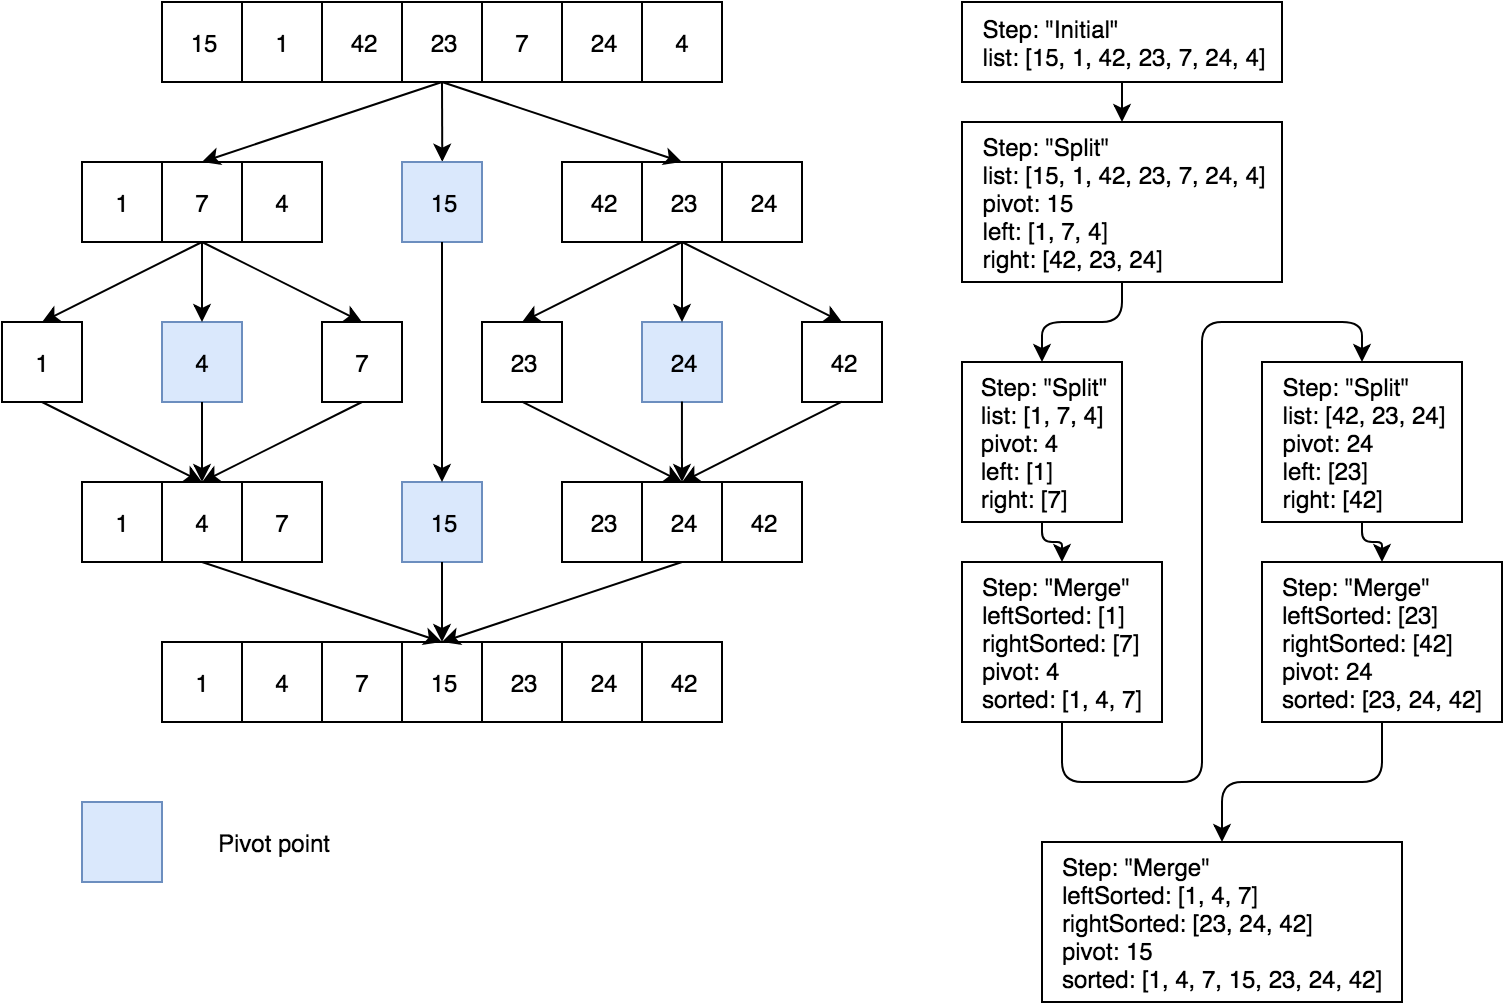
\includegraphics[width=\linewidth]{/diagrammer/Quicksort}
    \caption{Quicksort}
    \label{fig:quicksort}
\end{figure}

    %Tree datastructures
    \section{Tree datastructures}

    \subsection{Binary Tree}
A binary tree data structure is a simple data structure whose structure resembles a tree. A binary tree consists of nodes each having an unique value. Each node has a reference to its parent node and its children nodes. The previous node that links to the current node is called a parent node. The child nodes are the next nodes in line after the current selected node. A tree node can only have up to 2 children node, and every node must have only 1 parent node. The exception to this rule is the very first node in the tree, which is called the root node. There can only be 1 root node in the tree. Since a node can only have up to 2 children nodes, the child nodes are usually referred to as either the left child node or the right child node. A node that has no child nodes will always be at the bottom of the tree, and are referred as leaf nodes. The binary tree data structure is notably used as file systems.\cite{BinaryTree} 

    \subsection{Binary Search Tree}
A Binary Search Tree(BST) tree is an evolved form of Binary Tree, that structured in a way that is more beneficial for storing large amounts of data. The criterias for a Binary tree to be a binary search tree is the following conditions:
\begin{itemize}
	\item{All left children nodes needs to have a value lower than its parent node.}
	\item{All right children nodes needs to have a value higher than its parent node.}
	\item{There cannot be any nodes with duplicate values in the tree.}
\end{itemize}
Having these requirements helps the BST search for the correct node, since the time it takes to find the correct node is shorten tremendously. Inserting new nodes in the tree is also quite simple, just traverse the tree, where the direction is dependent on the new nodes value. Once a leaf node has been reached, put it as either a left child or a right child based on whether the new node's value is lower or greater than the lead node's value.\cite{BinaryTree,BST}

    \subsection{AVL}
%Note might have to change all avl trees to just avl
An AVL tree is a binary search tree, that can balance itself when it is needed. An AVL tree has only one additional condition compared to a normal BST. AVL trees can only have a height of one or lower difference between the left and right subtree in any of the nodes in the tree. This means for instance that a node that has a left subtree of height one and a right subtree of height three is not a qualified subtree. In order to keep this height balance between the subtrees, the AVL tree has to rebalance itself by rotating in either the left or right direction.
\\[11pt]
There are four different rotations that can be performed:
\begin{itemize}
    \item{Left}
    \item{Right}
    \item{Double Left, also referred to as right left rotation}
    \item{Double Right, also referred to as left right rotation}
\end{itemize}


    % Python
    \subsection{Python}
Python is the programming language used in the DAT100 course at UiS. Students are often struggeling to understand the difference between value type and reference type variables. To make it easier for them to learn, a Python interpreter was implemented which evaluates Python code step by step. Together with the GraphDrawer, the interpreter can be used to ask questions about Python code. The student is able to see whether a variable is value or reference type, and they can see when the value or reference changes. Before implementing a custom interpreter, using the offical Python interpreter was considered. Because of the size of CPython, and the limited time available for this project, it was decided that implementing a custom interpreter was the better option.
\\[11pt]
The following features of Python are supported:
\begin{enumerate}
    \item Variables of the following types: Number, String, Boolean, and Object.
    \item Functions can be defined using the \code{def} keyword. They can either belong to the global scope, or to a class. Functions can return something using the \code{return} keyword.
    \item Classes can be defined using the \code{class} keyword. If a function with the \code{__init__} is defined inside the class, it will be called when a new instance of the class is instantiated.
    \item If statements can be used with the \code{if} keyword. Elif and else statements are also supported.
    \item The following mathematical operators are supported: +, -, /, *.
    \item The following comparison operators are supported: and, or, !, ==, !=, <, >, >=, <=.
    \item Expressions can be grouped and seperated using parenthesis.
    \item Lines starting with a # are treated as comments, and will be skipped by the interpreter.
\end{enumerate}
Significant Python features missing from this interpreter:
\begin{enumerate}
    \item The standard library.
    \item Lists and dictionaries.
    \item Inner classes and functions.
    \item Shared class variables.
    \item Class inheritance.
    \item Loops.
\end{enumerate}
Every operator has the same priority, which means that expressions are always evaluated left to right. This makes some expressions not behave like expected. The following statement results in an error: \code{if 1 + 1 == 2:}, because it is evaluated as \code{1 + (1 == 2)}. To prevent this from happening, parenthesis should be used to order the expressions. The correct statement would be: \code{if (1 + 1) == 2:}.

\subsubsection{Interpreter}
There are three main functions in the interpreter. \code{parseLine} which tries to figure out what the meaning of a code line is. \code{parseLine} is also responsible for deciding which line to parse next. A line can either be a variable assignment which is handled  by the \code{parseLine} function, an expression which is handled by the \code{evaluateExpression} function, or a statement which is handled by the \code{handleKeyword} function. A statement is anything which starts with one of the keywords. An expression is something which can be evaluated to a value.
!! Insert fancy image showing the path code goes trough the interpreter !!
\\[11pt]
An important feature of the interpreter is the scope objects. A scope is an object which stores information about the variables, classes, functions and data inside the scope. Functions are scopes because they can contain private variables. Classes are also scopes, because they can contain functions. Before code can be parsed, a global scope is created. Anything which doesn't belong to a specific scope, is placed in the global scope. Scope data is an array where the index is the address of the stored data, and the value is the stored data. Because the interpreter is implemented in JavaScript, there is no need to seperate value and references types in this array because JavaScript and Python behave the same way. Scope variables are a mapping from variable names to data addresses. Scope functions/classes are mappings from function/class names to function/class objects. Because the interpreter should save the state of the program as steps, the \code{parseLine} function returns an object containing information about the state. If the state was anything other than a function or class definition, the current state is saved as a step.
\\[11pt]
A function is an object with a \code{name}, a list of arguments \code{args}, a list of the code lines belonging to the function \code{code}. A function should also be a scope. The name is used to identify the function. The arguments are used to make sure that when the function is called, the right amount of arguments are passed. The code is stored so the function can be evaluated when it is called. After a function has been defined, the \code{handleKeyword} function returns a state of type \code{"SkipLines"} which tells the caller which lines have already been handled. The interpreter uses the \code{callFunc} function to call Python functions. When a function is called, three things happen in the following order:
\begin{enumerate}
    \item The function arguments are added as local variables. Local variables mean they belong to the function scope. The arguments need to be in the same order as they were defined, because named arguments are not implemented.
    \item Every line found in the functions \code{code} list is parsed using \code{parseLine}. If a \code{return} statement is found before reaching the end, the function will stop parsing, before reaching the end.
    \item The scope of the function is restored to an empty state and data is returned if a return statement was found.
\end{enumerate}
\\[11pt]
A class is an object with a \code{name} and a list of the code lines belonging to the class \code{code}. A class should also be a scope. When a class is defined, the code is also parsed using the \code{parseLine} function. This is done so that any functions within the class is defined in the scope of the class. When the interpreter is instantiating an instance of the class, the \code{instantiateClass} function is called. \code{instantiateClass} will first create a new object which contains all the functions from the class. If the class has a constructor it is called. Finally, the object is returned to the called of \code{instantiateClass}.
!! Write about expression evaluation !!
!! Write about operators !!

\subsubsection{Questions}
!! TODO: Write this :=) !!

\end{appendices}

	\end{spacing}
\end{document}
